\documentclass[10pt]{beamer}
\usefonttheme{professionalfonts}
%\usetheme{CambridgeUS}
%
% Choose how your presentation looks.
%
% For more themes, color themes and font themes, see:
% http://deic.uab.es/~iblanes/beamer_gallery/index_by_theme.html
%
\mode<presentation>
{
  \usetheme{default}      % or try Darmstadt, Madrid, Warsaw, ...
  \usecolortheme{beaver} % or try albatross, beaver, crane, ...
  \usefonttheme{default}  % or try serif, structurebold, ...
  \setbeamertemplate{navigation symbols}{}
  \setbeamertemplate{caption}[numbered]
} 

\usepackage[english]{babel}
\usepackage[utf8x]{inputenc}
\usepackage{tikz}
\usepackage{pgfplots}
\usepackage{array}  % for table column M
\usepackage{makecell} % to break line within a cell
\usepackage{verbatim}
\usepackage{graphicx}
\usepackage{epstopdf}
\usepackage{amsfonts}
\usepackage{xcolor}
%\captionsetup{compatibility=false}
%\usepackage{dsfont}
\usepackage[absolute,overlay]{textpos}
\usetikzlibrary{calc}
\usetikzlibrary{pgfplots.fillbetween, backgrounds}
\usetikzlibrary{positioning}
\usetikzlibrary{arrows}
\usetikzlibrary{pgfplots.groupplots}
\usetikzlibrary{arrows.meta}
\usetikzlibrary{plotmarks}
\usetikzlibrary{calc}

\usepgfplotslibrary{groupplots}
\pgfplotsset{compat=newest} 
%\pgfplotsset{plot coordinates/math parser=false}

\usepackage{hyperref}
\hypersetup{
    colorlinks=true,
    linkcolor=blue,
    filecolor=magenta,      
    urlcolor=cyan,
}

\definecolor{matlabcomment}{RGB}{34,139,34}

\pgfmathdeclarefunction{gauss}{2}{%
	\pgfmathparse{1/(#2*sqrt(2*pi))*exp(-((x-#1)^2)/(2*#2^2))}%
}

\pgfmathdeclarefunction{laplacian}{2}{%
	\pgfmathparse{1/(#2*2)*exp(-(abs(x-#1))/(#2))}%
}

\tikzset{
	declare function={
		sign(\x) = (and(\x<0, 1) * -1) +
		(and(\x>0, 1) * 1);
}
}

\pgfmathdeclarefunction{invgauss}{2}{%
	\pgfmathparse{sqrt(-2*ln(#1))*cos(deg(2*pi*#2))}%
}

\DeclareMathOperator{\E}{\mathbb{E}} % expectation

\newcolumntype{M}[1]{>{\centering\arraybackslash}m{#1}}

\definecolor{blue2}{RGB}{51, 105, 232}  
\definecolor{red2}{RGB}{213, 15, 37}  
\definecolor{green2}{RGB}{0, 153, 37}  
\definecolor{green3}{rgb}{0.1922, 0.6392, 0.3294}% 
\definecolor{yellow2}{RGB}{238, 178, 17} 
\definecolor{gray2}{RGB}{102, 102, 102}
\definecolor{orange2}{RGB}{230, 85, 13}

% Qualitative pallete set1 from www.ColorBrewer.org
\definecolor{Qred}{RGB}{228,26,28}
\definecolor{Qblue}{RGB}{55,126,184}
\definecolor{Qgreen}{RGB}{77,175,74}
\definecolor{Qpurple}{RGB}{152,78,163}
\definecolor{Qorange}{RGB}{255,127,0}
\definecolor{Qyellow}{RGB}{255,255,51}
\definecolor{Qbrown}{RGB}{166,86,40}
\definecolor{Qpink}{RGB}{247,129,191}
\definecolor{Qgray}{RGB}{153,153,153}

\title[EE 264]{Discrete-Time Random Signals}
\author{Jose Krause Perin}
\institute{Stanford University}
\date{July 29, 2017}

\begin{document}

\begin{frame}
  \titlepage
\end{frame}

% Uncomment these lines for an automatically generated outline.
%\begin{frame}{Outline}
%  \tableofcontents
%\end{frame}

\begin{frame}{Announcements}

\begin{itemize}
	\item If you're enrolled for 4 units, don't forget to adjust your units on Axess and enroll for 3 units. \textbf{Deadline:} July 7
	\item Homework 1 will be released today and it is due next Thursday
	\item No lecture or office hours next Tuesday (Independence Day)
\end{itemize}

\end{frame}

\begin{frame}{Last lecture}

\begin{block}{Review of discrete-time signals and systems}
	\begin{itemize}
		\item Systems can be linear, time-invariant, memoryless, causal, and stable \\
		\item LTI systems are completely characterized by their impulse response \\
		\item We can use the convolution sum to calculate the output of an LTI system to any signal \\
		\item The complex exponential $e^{j\omega n}$, and more generally $z^n$, are eigenfunctions of LTI systems
		\item Frequency-domain representation of signals and systems
		\begin{itemize}
			\item DTFT
			\item $z$-transform and ROC. Without the ROC the $z$-transform is ambiguous
		\end{itemize}
		\item The DTFT is equivalent to the $z$-transform evaluated on the unit circle: $H(e^{j\omega}) = H(z = e^{j\omega})$, provided that the unit circle is in the ROC of the $z$-transform
	\end{itemize}
\end{block}

\end{frame}

\section{Introduction}
\begin{frame}{Today's lecture} 

How to analyze LTI systems when the input is a random signal?

\begin{block}{Motivation}
	\begin{itemize}
		\item Many signals vary in complicated patterns that
		cannot be easily described analytically
		\item It is often convenient and useful to consider
		such signals as being created by some sort of
		random mechanism
	\end{itemize}   	
\end{block}
\end{frame}

%
\begin{frame}{Example: speech signals}

Speech signals are well described by the \textbf{Laplacian distribution}

\begin{figure}
	\centering
	\resizebox{\linewidth}{!}{\begin{tikzpicture}
\begin{axis}[%
name=speech,
axis lines*=middle,
xlabel=$t$,
ylabel=$x(t)$,
scale only axis,
axis on top,
%separate axis lines,
% every outer x axis line/.append style={white!15!black},
% every x tick label/.append style={font=\color{white!15!black}},
xmin=3364,
xmax=10100,
ytick=\empty,
xtick=\empty,
axis line style={->,>=stealth},
every axis x label/.style={
	at={(ticklabel* cs:0.97)},
	anchor=north,
},
every axis y label/.style={
	at={(ticklabel* cs:1)},
	anchor=south,
},
every axis y label/.style={at=(current axis.above origin),anchor=south},
%every axis x label/.style={at=(current axis.right of origin),anchor=west},
ymin=-1,
ymax=1,
]
\addplot [line width = 1.5pt, color=blue2!90] table [x={time}, y={sound}] {figs/speech_data.dat};
\end{axis}

\onslide<2|handout:1>{
\begin{axis}[
at=(speech.east), %anchor=east,
anchor=origin,
%at={(1200,380)},
xmin=-5,
xmax=5,
width=3.5in,
height=2in,
no markers,
rotate around={-90:(current axis.origin)}, % Rotate around the origin
axis lines*=center,
every axis y label/.style={at=(current axis.above origin),anchor=south},
every axis x label/.style={at=(current axis.right of origin),anchor=west},
%height=5cm, width=8cm,
xtick=\empty,
ymin=0,
ymax=0.6,
ytick=\empty,
xlabel=$x$,
ylabel=$p_{x(t)}(x)$,
enlargelimits=false, clip=false, axis on top,
grid = major,
axis line style={->,>=stealth},
every axis x label/.style={
	at={(ticklabel* cs:0)},
	xshift=0.3cm,
	anchor=north,
},
every axis y label/.style={
	at={(ticklabel* cs:1)},
	anchor=south,
},
x dir=reverse,
]
\addplot [very thick,black, fill=blue2!70,domain=-5:5, samples=101, clip=true] {laplacian(0,0.9)};
\node at (axis cs: 3, 0.5) {$\displaystyle p_{x(t)}(x) = \frac{1}{2b}\exp\bigg(-\frac{|x-\mu|}{b}\bigg)$};
\end{axis}
}
\end{tikzpicture}%}
	\label{fig:speech_and_dist}
\end{figure} 

\end{frame}


%
\begin{frame}{Example: quantization}

Quantization error is well described by an \textbf{uniform distribution}, even though quantization is a deterministic operation 
\vspace{-0.6cm}
\begin{center}
	\resizebox{\linewidth}{!}{\def\H{0.3\textwidth}
\def\W{0.7\textwidth}

\begin{tikzpicture}
\onslide<1|handout:1>{
\begin{axis}[
name=plot1a,
axis lines*=middle,
enlargelimits = true,
width=\W,
height=\H,
clip=true,
scale only axis,
axis line style={->,>=stealth},
xlabel={\small $n$},
ylabel={\small $x[n]$},
every axis x label/.style={
	at={(ticklabel* cs:1)},
	xshift=-0.2cm,
	anchor=north,
},
every axis y label/.style={
	at={(ticklabel* cs:1)},
	xshift=0.4cm,
	yshift=-0.35cm,
	anchor=south,
},
every outer x axis line/.append style={white!15!black},
every x tick label/.append style={font=\color{white!15!black}},
xmin=1.00,
xmax=50.00,
ymin=-25.00,
ymax=25.00,
ytick=\empty,
xtick=\empty,
yticklabel=\empty,
xmajorgrids,
ymajorgrids,
every outer y axis line/.append style={white!15!black},
every y tick label/.append style={font=\color{white!15!black}},
legend style={draw=white!15!black,fill=white,legend cell align=left}]
\addplot [smooth, black, mark=*, mark options={scale=0.75, fill=white}, line width=1.5pt, forget plot]
table[row sep=crcr]{
	1 -6.3246 \\
2 0.14148 \\
3 14.2497 \\
4 -0.47482 \\
5 2.0162 \\
6 4.5187 \\
7 3.3055 \\
8 5.938 \\
9 -2.9003 \\
10 1.9589 \\
11 4.2128 \\
12 -5.5237 \\
13 -1.7526 \\
14 -4.3109 \\
15 -12.5332 \\
16 6.5333 \\
17 11.3842 \\
18 -5.9984 \\
19 -5.873 \\
20 5.874 \\
21 2.1636 \\
22 -7.5453 \\
23 9.2793 \\
24 -3.5217 \\
25 -24.2767 \\
26 -6.1509 \\
27 -2.9481 \\
28 -3.54 \\
29 0.28986 \\
30 -2.472 \\
31 -2.0041 \\
32 0.97429 \\
33 -1.2649 \\
34 2.4889 \\
35 8.7989 \\
36 8.1063 \\
37 8.627 \\
38 2.4047 \\
39 9.3665 \\
40 5.4453 \\
41 -4.6892 \\
42 -5.4897 \\
43 -9.1199 \\
44 11.6971 \\
45 7.0293 \\
46 -9.2606 \\
47 -7.9473 \\
48 -9.7386 \\
49 3.7947 \\
50 5.967 \\
};
\end{axis}
}

\onslide<2|handout:2>{
	\begin{axis}[
	name=plot1a,
	axis lines*=middle,
	enlargelimits = true,
	width=\W,
	height=\H,
	clip=true,
	scale only axis,
	axis line style={->,>=stealth},
	xlabel={\small $n$},
	ylabel={\small $x[n]$},
	every axis x label/.style={
		at={(ticklabel* cs:1)},
		xshift=-0.2cm,
		anchor=north,
	},
	every axis y label/.style={
		at={(ticklabel* cs:1)},
		xshift=0.4cm,
		yshift=-0.35cm,
		anchor=south,
	},
	every outer x axis line/.append style={white!15!black},
	every x tick label/.append style={font=\color{white!15!black}},
	xmin=1.00,
	xmax=50.00,
	ymin=-25.00,
	ymax=25.00,
	yticklabels=\empty,
	xtick=\empty,
	ytick ={-24.2767,  -17.3405,  -10.4043,   -3.4681  ,  3.4681,   10.4043,   17.3405,   24.2767},
	xmajorgrids,
	ymajorgrids,
	every outer y axis line/.append style={white!15!black},
	every y tick label/.append style={font=\color{white!15!black}},
	legend style={draw=white!15!black,fill=white,legend cell align=left}]
	\addplot [smooth, black, mark=*, mark options={scale=0.75, fill=white}, line width=1.5pt, forget plot]
	table[row sep=crcr]{
		1 -6.3246 \\
		2 0.14148 \\
		3 14.2497 \\
		4 -0.47482 \\
		5 2.0162 \\
		6 4.5187 \\
		7 3.3055 \\
		8 5.938 \\
		9 -2.9003 \\
		10 1.9589 \\
		11 4.2128 \\
		12 -5.5237 \\
		13 -1.7526 \\
		14 -4.3109 \\
		15 -12.5332 \\
		16 6.5333 \\
		17 11.3842 \\
		18 -5.9984 \\
		19 -5.873 \\
		20 5.874 \\
		21 2.1636 \\
		22 -7.5453 \\
		23 9.2793 \\
		24 -3.5217 \\
		25 -24.2767 \\
		26 -6.1509 \\
		27 -2.9481 \\
		28 -3.54 \\
		29 0.28986 \\
		30 -2.472 \\
		31 -2.0041 \\
		32 0.97429 \\
		33 -1.2649 \\
		34 2.4889 \\
		35 8.7989 \\
		36 8.1063 \\
		37 8.627 \\
		38 2.4047 \\
		39 9.3665 \\
		40 5.4453 \\
		41 -4.6892 \\
		42 -5.4897 \\
		43 -9.1199 \\
		44 11.6971 \\
		45 7.0293 \\
		46 -9.2606 \\
		47 -7.9473 \\
		48 -9.7386 \\
		49 3.7947 \\
		50 5.967 \\
	};
	\end{axis}
}

\onslide<3-|handout:3>{
\begin{axis}[
name=plot1,
axis lines*=middle,
enlargelimits = true,
width=\W,
height=\H,
clip=true,
scale only axis,
axis line style={->,>=stealth},
xlabel={\small $n$},
%ylabel={\small $x[n]$},
every axis x label/.style={
	at={(ticklabel* cs:1)},
	xshift=-0.2cm,
	anchor=north,
},
every axis y label/.style={
	at={(ticklabel* cs:1)},
	xshift=0.1cm,
	anchor=south,
},
every outer x axis line/.append style={white!15!black},
every x tick label/.append style={font=\color{white!15!black}},
xmin=1.00,
xmax=50.00,
ymin=-25.00,
ymax=25.00,
ytick ={-24.2767,  -17.3405,  -10.4043,   -3.4681  ,  3.4681,   10.4043,   17.3405,   24.2767},
xtick=\empty,
yticklabel=\empty,
xmajorgrids,
ymajorgrids,
every outer y axis line/.append style={white!15!black},
every y tick label/.append style={font=\color{white!15!black}},
legend style={draw=white!15!black,fill=white,scale=0.3,legend cell align=left, at={(axis cs: 47,10)},anchor=south west}]
\addplot [smooth, black!30, mark=*, mark options={scale=0.75, fill=white}, line width=1.5pt]
table[row sep=crcr]{
	1 -6.3246 \\
2 0.14148 \\
3 14.2497 \\
4 -0.47482 \\
5 2.0162 \\
6 4.5187 \\
7 3.3055 \\
8 5.938 \\
9 -2.9003 \\
10 1.9589 \\
11 4.2128 \\
12 -5.5237 \\
13 -1.7526 \\
14 -4.3109 \\
15 -12.5332 \\
16 6.5333 \\
17 11.3842 \\
18 -5.9984 \\
19 -5.873 \\
20 5.874 \\
21 2.1636 \\
22 -7.5453 \\
23 9.2793 \\
24 -3.5217 \\
25 -24.2767 \\
26 -6.1509 \\
27 -2.9481 \\
28 -3.54 \\
29 0.28986 \\
30 -2.472 \\
31 -2.0041 \\
32 0.97429 \\
33 -1.2649 \\
34 2.4889 \\
35 8.7989 \\
36 8.1063 \\
37 8.627 \\
38 2.4047 \\
39 9.3665 \\
40 5.4453 \\
41 -4.6892 \\
42 -5.4897 \\
43 -9.1199 \\
44 11.6971 \\
45 7.0293 \\
46 -9.2606 \\
47 -7.9473 \\
48 -9.7386 \\
49 3.7947 \\
50 5.967 \\
}; \addlegendentry{$x[n]$};

\addplot [ycomb, red, mark=*, mark options={scale=0.75, fill=white}, line width=1.5pt]
table[row sep=crcr]{
	1 -3.4681 \\
2 3.4681 \\
3 17.3405 \\
4 -3.4681 \\
5 3.4681 \\
6 3.4681 \\
7 3.4681 \\
8 3.4681 \\
9 -3.4681 \\
10 3.4681 \\
11 3.4681 \\
12 -3.4681 \\
13 -3.4681 \\
14 -3.4681 \\
15 -10.4043 \\
16 3.4681 \\
17 10.4043 \\
18 -3.4681 \\
19 -3.4681 \\
20 3.4681 \\
21 3.4681 \\
22 -10.4043 \\
23 10.4043 \\
24 -3.4681 \\
25 -24.2767 \\
26 -3.4681 \\
27 -3.4681 \\
28 -3.4681 \\
29 3.4681 \\
30 -3.4681 \\
31 -3.4681 \\
32 3.4681 \\
33 -3.4681 \\
34 3.4681 \\
35 10.4043 \\
36 10.4043 \\
37 10.4043 \\
38 3.4681 \\
39 10.4043 \\
40 3.4681 \\
41 -3.4681 \\
42 -3.4681 \\
43 -10.4043 \\
44 10.4043 \\
45 10.4043 \\
46 -10.4043 \\
47 -10.4043 \\
48 -10.4043 \\
49 3.4681 \\
50 3.4681 \\
}; \addlegendentry{$x_Q[n] = \big[x[n]\big]_Q$};
\end{axis}
}
\onslide<4-|handout:3>{
\begin{axis}[
name=plot2,
at=(plot1.below south east), anchor=above north east,
axis lines*=middle,
enlargelimits = true,
clip=true,
width=\W,
height=\H,
scale only axis,
axis line style={->,>=stealth},
xlabel={\small $n$},
ylabel={\small $\epsilon[n] = \frac{x[n]-x_Q[n]}{\Delta x}$},
every axis x label/.style={
	at={(ticklabel* cs:1)},
	xshift=-0.2cm,
	anchor=north,
},
every axis y label/.style={
	at={(ticklabel* cs:1)},
	xshift=0.1cm,
	anchor=south,
},
every outer x axis line/.append style={white!15!black},
every x tick label/.append style={font=\color{white!15!black}},
xmin=1.00,
xmax=50.00,
ymin=-0.5,
ymax=0.5,
ytick ={-0.5, 0.5},
xtick=\empty,
%yticklabel=\empty,
xmajorgrids,
ymajorgrids,
every outer y axis line/.append style={white!15!black},
every y tick label/.append style={font=\color{white!15!black}},
legend style={draw=white!15!black,fill=white,legend cell align=left}]
\addplot [ycomb, mark=*, fill=white, mark options={scale=0.75, fill=white}, line width=1.5pt, forget plot]
table[row sep=crcr]{
	1 -0.41182 \\
2 -0.4796 \\
3 -0.4456 \\
4 0.43154 \\
5 -0.20932 \\
6 0.15146 \\
7 -0.023437 \\
8 0.35608 \\
9 0.081859 \\
10 -0.21758 \\
11 0.10736 \\
12 -0.29636 \\
13 0.24732 \\
14 -0.1215 \\
15 -0.30693 \\
16 0.44191 \\
17 0.14128 \\
18 -0.3648 \\
19 -0.34672 \\
20 0.34687 \\
21 -0.18807 \\
22 0.41218 \\
23 -0.16219 \\
24 -0.0077354 \\
25 0 \\
26 -0.38678 \\
27 0.074972 \\
28 -0.01037 \\
29 -0.45821 \\
30 0.1436 \\
31 0.21106 \\
32 -0.35954 \\
33 0.31764 \\
34 -0.14117 \\
35 -0.23145 \\
36 -0.3313 \\
37 -0.25624 \\
38 -0.15331 \\
39 -0.14962 \\
40 0.28506 \\
41 -0.17604 \\
42 -0.29146 \\
43 0.18517 \\
44 0.18638 \\
45 -0.48658 \\
46 0.16489 \\
47 0.35423 \\
48 0.095976 \\
49 0.047092 \\
50 0.36027 \\
};
\end{axis}
}
\onslide<5|handout:3>{
\begin{axis}[
at=(plot2.east), %anchor=east,
anchor=origin,
%at={(1200,380)},
xmin=-0.5,
xmax=0.5,
width=1.89in,
height=1.5in,
no markers,
rotate around={-90:(current axis.origin)}, % Rotate around the origin
axis lines*=center,
every axis y label/.style={at=(current axis.above origin),anchor=south},
every axis x label/.style={at=(current axis.right of origin),anchor=west},
%height=5cm, width=8cm,
xtick=\empty,
ytick=\empty,
xticklabel=\empty,
ymin=0,
ymax=1.2,
yticklabel style = {xshift=0.4cm, yshift=-0.2cm},
ylabel=$p_{\epsilon[n]}(e)$,
xlabel={$e$},
enlargelimits=true, clip=true, axis on top,
grid = major,
axis line style={->,>=stealth},
every axis x label/.style={
	at={(ticklabel* cs:0)},
	yshift=0.2cm,
	xshift=0.2cm,
	anchor=north,
},
every axis y label/.style={
	at={(ticklabel* cs:1)},
	anchor=south,
	xshift=0.3cm,
},
x dir=reverse,
]
\addplot[black, ybar interval, fill=black!20, mark=no] plot coordinates { (-0.475000, 0.996875) (-0.425000, 1.050000) (-0.375000, 0.987500) (-0.325000, 1.112500) (-0.275000, 1.087500) (-0.225000, 1.003125) (-0.175000, 0.996875) (-0.125000, 1.043750) (-0.075000, 1.006250) (-0.025000, 1.009375) (0.025000, 0.984375) (0.075000, 0.975000) (0.125000, 0.890625) (0.175000, 1.056250) (0.225000, 0.990625) (0.275000, 0.975000) (0.325000, 0.962500) (0.375000, 0.900000) (0.425000, 0.978125) (0.475000, 0.993750) };
\addplot [very thick, black, clip=true] coordinates {(-0.6,0) (-0.5, 0) (-0.5, 1) (0.5, 1) (0.5, 0) (0.6, 0)};
\end{axis}
}
\end{tikzpicture}}
\end{center}

\onslide<5>{More about quantization in lectures 5 and 8.}

\end{frame}

%
\begin{frame}{Example: noise and interference}

Noise and interfering signals are typically modeled as \textbf{random processes}

\begin{enumerate}
	\item What's the effect of the noise on the output? 
	\item How can we design the system to minimize the noise at the output?	
\end{enumerate}

\begin{figure}
	\centering
	\resizebox{\linewidth}{!}{\def\layersep{1.5cm}
\def\outsep{0.7cm}
\def\dy{1}

\begin{tikzpicture}[->, >=stealth, shorten >= 0pt, draw=black!50, node distance=\layersep, font=\sffamily]
    \tikzstyle{node}=[circle,fill=black,minimum size=2pt,inner sep=0pt]
    \tikzstyle{block}=[draw=black,rectangle,fill=none,minimum size=1.5cm, inner sep=0pt]
    \tikzstyle{summer}=[draw=black,circle,fill=none,minimum size=1cm, inner sep=0pt]
    \tikzstyle{annot} = []

	\node[node] (sc) at (0, -\dy cm) {};
	\node[summer] (add) at (1*\layersep, -\dy cm) {\Large $+$};
	\node[node, below=\dy cm of add] (nc) {};
    \node[block] (DSP) at ($(add.east) + (\layersep, 0)$) {System};
	\coordinate (yc) at ($(DSP.center) + (\layersep, 0)$) {};
	
	%\coordinate (mid1) at ($(ADC.east)!0.5!(DSP.west)$) {};
	%\coordinate (mid2) at ($(DSP.east)!0.5!(DAC.west)$) {};
		
    \path (sc) edge (add);
    \path (add) edge (DSP);
    \path (nc) edge (add);
    \path (DSP) edge (yc);
    
    \node[left = 0mm of sc, text width = 1cm, align=center] {Signal};
    \node[right = 0mm of yc, text width = 1cm, align=center] {Output}; 
    \node[below = 0mm of nc, text width = 2cm, align=center] {Noise or \\ interference};
    

\end{tikzpicture}}
\end{figure} 
\end{frame}

\begin{frame}{Outline}

\textbf{Our goal:} analyze LTI systems when the input signal is random

\begin{enumerate}
	\item Random processes
	\begin{itemize}
		\item Averages of a random variable
		\item Stationary random processes
		\item Time averages and ergodic random processes
	\end{itemize}
	\item LTI systems with a random input
	\item White noise
	\item Examples
\end{enumerate}
\end{frame}

%
\section{Random processes}
\begin{frame}{Random processes}

\begin{block}{Definition}
	A random process (or \textit{stochastic process}) is an indexed set of random variables $x_n$, which are distributed according to some probability distribution $p_{x_n}(x)$
\end{block}	

\begin{block}{Examples}
\begin{columns}
	\begin{column}{0.5\textwidth}
		Consecutive coin tosses
	\end{column}
	\begin{column}{0.5\textwidth}  %%<--- here
		Random bit stream
	\end{column}
\end{columns}

\begin{columns}
	\begin{column}{0.5\textwidth}
		\begin{tikzpicture}[draw=black!50, node distance=1cm]
		\tikzstyle{block}=[draw=none,rectangle,fill=none,minimum size=1.5cm, inner sep=0pt]
		\node[block] (C1) {\resizebox{1.5cm}{!}{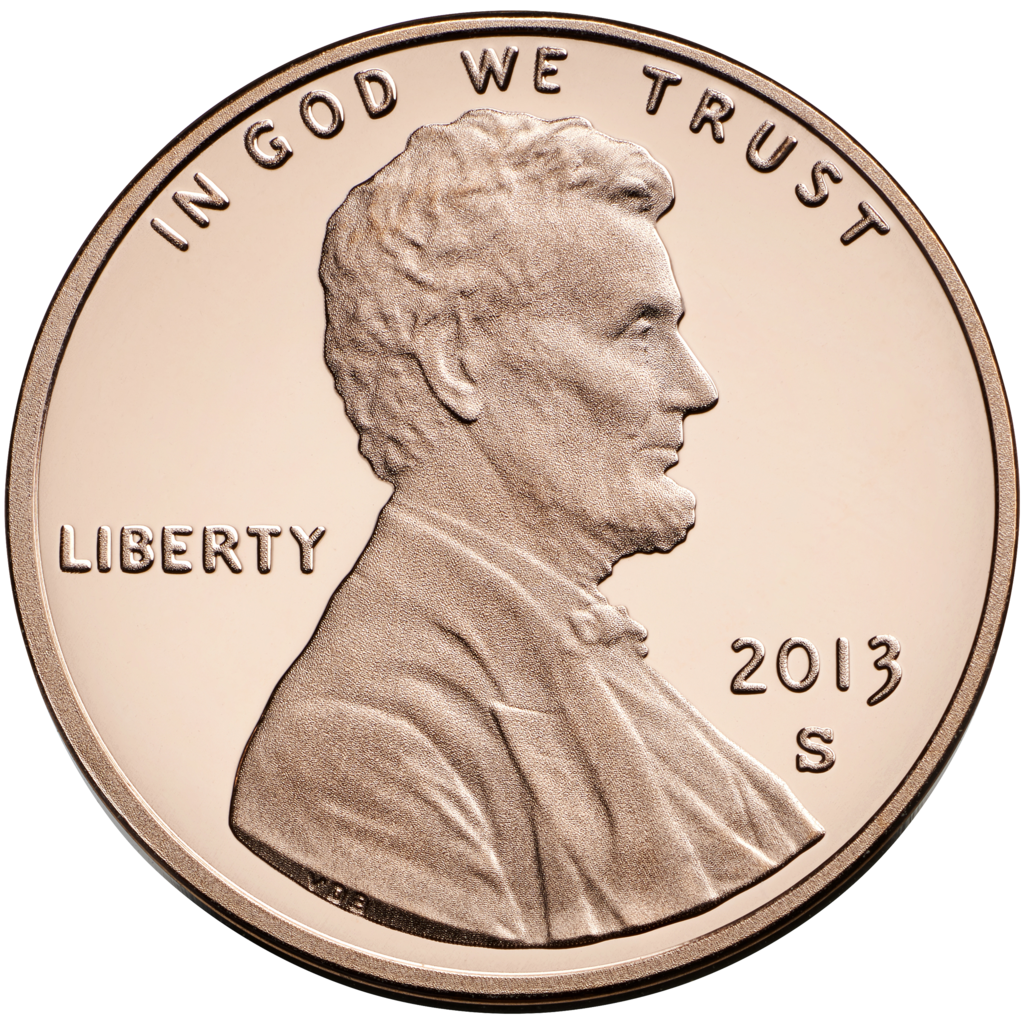
\includegraphics{figs/US_One_Cent_Obv.png}}};
		\node[block,right of=C1] (C2) {\resizebox{1.5cm}{!}{
\includegraphics{figs/US_One_Cent_Rev.png}}};
		\node[block,right of=C2] (C3) {\resizebox{1.5cm}{!}{
\includegraphics{figs/US_One_Cent_Rev.png}}};
		\node[block,right of=C3] (C4) {\resizebox{1.5cm}{!}{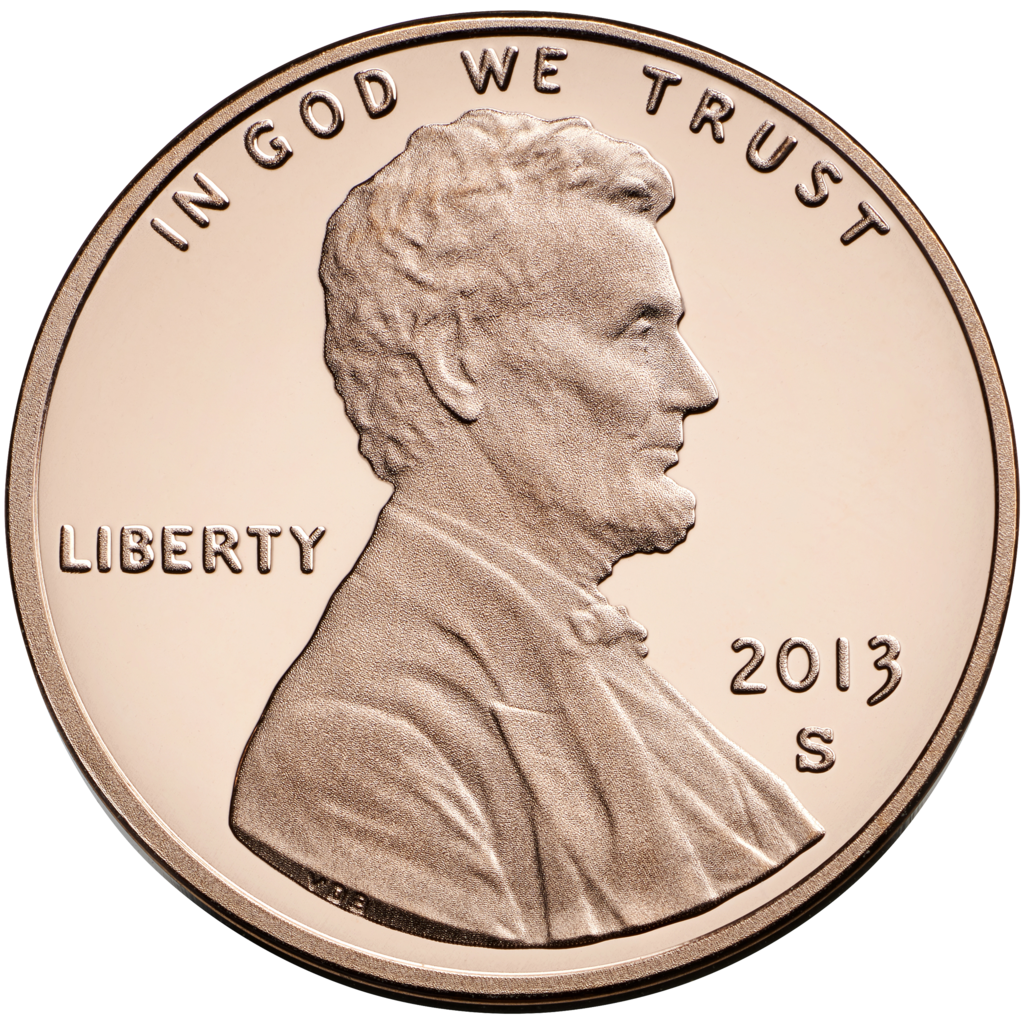
\includegraphics{figs/US_One_Cent_Obv.png}}};
		\node[block,right of=C4] (C5) {\Large$~~~\cdots$};
		\end{tikzpicture}
	\end{column}
	\begin{column}{0.5\textwidth}  %%<--- here
		\resizebox{0.8\linewidth}{!}{\begin{tikzpicture} 
\begin{axis}[
axis lines*=middle,
enlargelimits = true,
clip=false,
%scale only axis,
width=\textwidth,
height=0.7\textwidth,
ymin=0,
ymax=1.1,
xmin=-5,
xmax=5,
axis line style={->,>=stealth},
xlabel={$n$},
ylabel={bits},
yticklabel style = {yshift=0.25cm},
xticklabel style = {yshift=-0.1cm},
every axis x label/.style={
    at={(ticklabel* cs:1)},
    anchor=north,
},
every axis y label/.style={
    at={(ticklabel* cs:1)},
    xshift=0.1cm,
    anchor=south,
},
%xtick=\empty,
ytick={1},
xtick=\empty,
%xtick={-3.14, -1, 1, 3.14},
%xticklabels={$-\pi$, $-\omega_c$, $\omega_c$, $\pi$},
%xmajorgrids,
%ymajorgrids,
every outer y axis line/.append style={white!15!black},
every y tick label/.append style={font=\color{white!15!black}},
legend style={draw=white!15!black,fill=white,legend cell align=left}]
\pgfmathsetseed{99}
\addplot[ycomb, mark=*, fill=white, mark options={scale=1, fill=white}, line width=1.5pt, domain=-5:5, samples=11] {0.5*(sign(rand)+1)};
\end{axis}
\end{tikzpicture}
}
	\end{column}
\end{columns}
\end{block}
\end{frame}

\begin{frame}{Random processes}
We can think of a random process as a function $X(n, \chi)$ of two variables, time $n$ and the outcome of the underlying random experiment $\chi$. 
\begin{itemize}
	\pause\item For fixed $n$, $X(n, \chi)$ is a random variable.
	
	In the example of the fair coin tossing, 
	\begin{equation*}
	X(n=1, \chi) = \begin{cases}
	\mathrm{H},~\text{with probability}~0.5 \\
	\mathrm{T},~\text{with probability}~0.5
	\end{cases}
	\end{equation*}
	\pause\item For fixed $\chi$, $X(n, \chi)$ is a deterministic function of $n$ called a \textbf{sample function} or \textbf{sample sequence}
	
	\vspace{3mm}
	\centering
	\begin{tikzpicture}[draw=black!50, node distance=1cm]
		\tikzstyle{block}=[draw=none,rectangle,fill=none,minimum size=1.5cm, inner sep=0pt]
		\node[block] (C1) {\resizebox{1.5cm}{!}{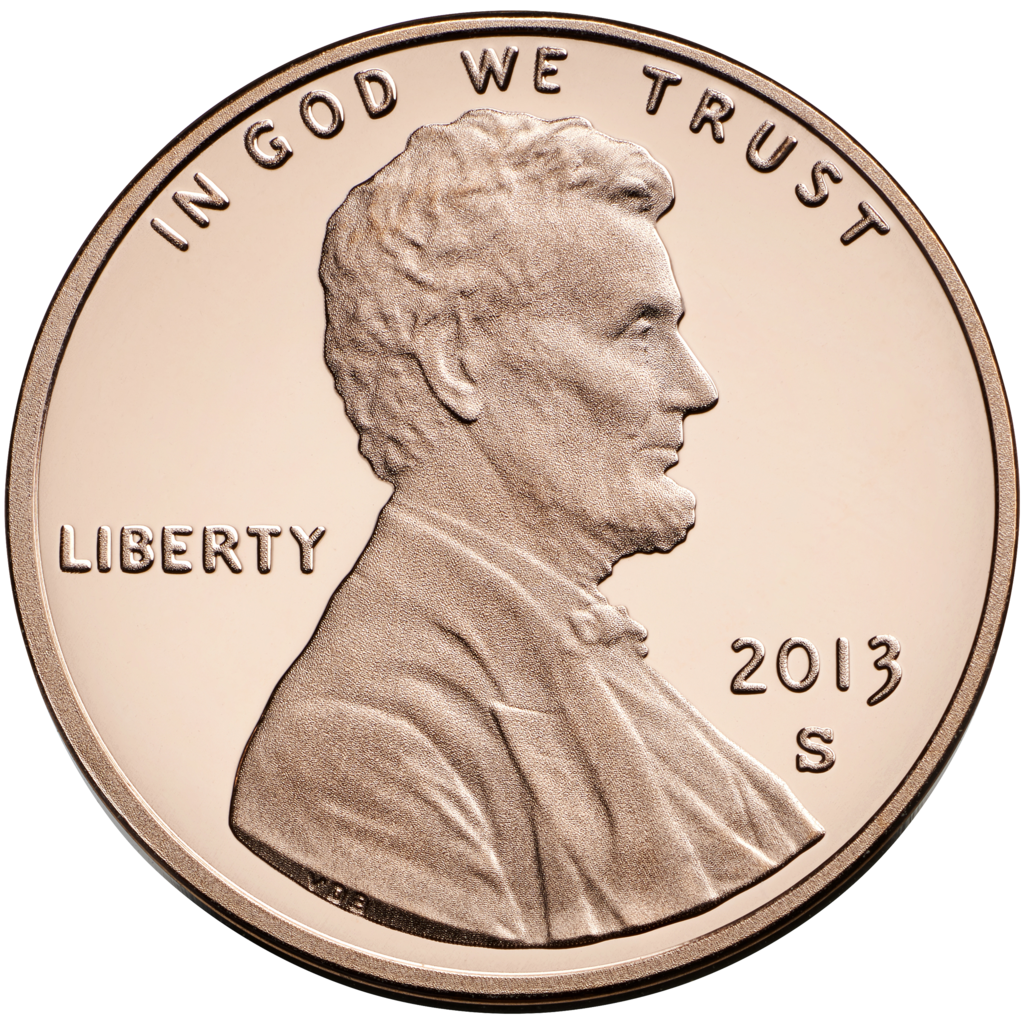
\includegraphics{figs/US_One_Cent_Obv.png}}};
		\node[block,right of=C1] (C2) {\resizebox{1.5cm}{!}{
\includegraphics{figs/US_One_Cent_Rev.png}}};
		\node[block,right of=C2] (C3) {\resizebox{1.5cm}{!}{
\includegraphics{figs/US_One_Cent_Rev.png}}};
		\node[block,right of=C3] (C4) {\resizebox{1.5cm}{!}{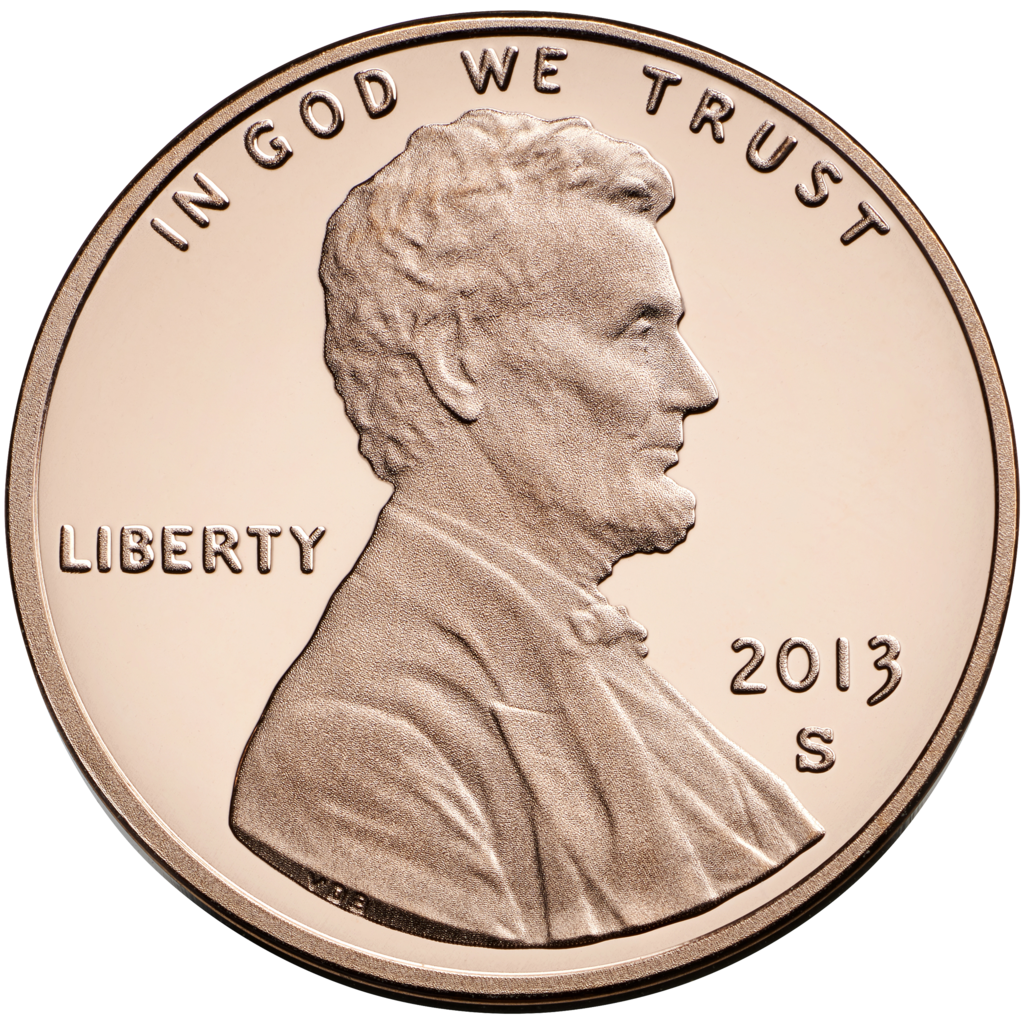
\includegraphics{figs/US_One_Cent_Obv.png}}};
		\node[block,right of=C4] (C5) {\Large$~~~\cdots$};
		\node[below of=C1, scale=0.7] (res1) {$X(1, \chi) = \mathrm{H}$};
		\node[below of=C4, scale=0.7] (res4) {$X(4, \chi) = \mathrm{H}$};
		\node[scale=0.7] at ($(res1.east)!0.5!(res4.west)$) {$\cdots$};
	\end{tikzpicture}
\end{itemize}
\end{frame}

\begin{frame}{Ensemble of sample sequences}
The ensemble of sample sequences is a collection af all sequences generated by a random process.
\vspace{-0.3cm}
\begin{center}
	\resizebox{0.8\linewidth}{!}{\def\W{6cm}
\def\H{2cm}
\begin{tikzpicture}[draw=black!50, node distance=0.3cm]
\pgfmathsetseed{99}
\tikzstyle{block}=[draw=none,rectangle,fill=none,inner sep=0pt]

\node[block] (s1) {\resizebox{0.1\linewidth}{!}{\begin{tikzpicture}
\begin{axis}[
	axis lines*=middle,
	enlargelimits = false,
	clip=false,
	scale only axis,
	hide y axis,
	width=0.5\textwidth,
	height=0.15\textwidth,
	ymin=-1.3,
	ymax=1.3,
	xmin=-11,
	xmax=11,
	axis line style={->,>=stealth},
	xlabel={\small $n$},
	every axis x label/.style={
		at={(ticklabel* cs:1)},
		xshift=0.2cm,
		anchor=north,
	},
	%xtick=\empty,
	ytick=\empty,
	xtick=\empty,
	%xtick={-3.14, -1, 1, 3.14},
	%xticklabels={$-\pi$, $-\omega_c$, $\omega_c$, $\pi$},
	%xmajorgrids,
	%ymajorgrids,
	every outer y axis line/.append style={white!15!black},
	every y tick label/.append style={font=\color{white!15!black}},
	legend style={draw=white!15!black,fill=white,legend cell align=left}]
	\addplot[ycomb, mark=*, fill=white, mark options={scale=0.75, fill=white}, line width=1pt, domain=-10:10, samples=21] {rand};
\end{axis}
\end{tikzpicture}
}};
\node[left=0cm of s1,scale=0.15] {$X(n, \chi_1)$};

\onslide<2->{
	\node[block, below of=s1] (s2) {\resizebox{0.1\linewidth}{!}{\begin{tikzpicture}
\begin{axis}[
	axis lines*=middle,
	enlargelimits = false,
	clip=false,
	scale only axis,
	hide y axis,
	width=0.5\textwidth,
	height=0.15\textwidth,
	ymin=-1.3,
	ymax=1.3,
	xmin=-11,
	xmax=11,
	axis line style={->,>=stealth},
	xlabel={\small $n$},
	every axis x label/.style={
		at={(ticklabel* cs:1)},
		xshift=0.2cm,
		anchor=north,
	},
	%xtick=\empty,
	ytick=\empty,
	xtick=\empty,
	%xtick={-3.14, -1, 1, 3.14},
	%xticklabels={$-\pi$, $-\omega_c$, $\omega_c$, $\pi$},
	%xmajorgrids,
	%ymajorgrids,
	every outer y axis line/.append style={white!15!black},
	every y tick label/.append style={font=\color{white!15!black}},
	legend style={draw=white!15!black,fill=white,legend cell align=left}]
	\addplot[ycomb, mark=*, fill=white, mark options={scale=0.75, fill=white}, line width=1pt, domain=-10:10, samples=21] {rand};
\end{axis}
\end{tikzpicture}
}};
	\node[left=0cm of s2,scale=0.15] {$X(n, \chi_2)$};
}

\onslide<3->{
	\node[block, below of=s2] (s3) {\resizebox{0.1\linewidth}{!}{\begin{tikzpicture}
\begin{axis}[
	axis lines*=middle,
	enlargelimits = false,
	clip=false,
	scale only axis,
	hide y axis,
	width=0.5\textwidth,
	height=0.15\textwidth,
	ymin=-1.3,
	ymax=1.3,
	xmin=-11,
	xmax=11,
	axis line style={->,>=stealth},
	xlabel={\small $n$},
	every axis x label/.style={
		at={(ticklabel* cs:1)},
		xshift=0.2cm,
		anchor=north,
	},
	%xtick=\empty,
	ytick=\empty,
	xtick=\empty,
	%xtick={-3.14, -1, 1, 3.14},
	%xticklabels={$-\pi$, $-\omega_c$, $\omega_c$, $\pi$},
	%xmajorgrids,
	%ymajorgrids,
	every outer y axis line/.append style={white!15!black},
	every y tick label/.append style={font=\color{white!15!black}},
	legend style={draw=white!15!black,fill=white,legend cell align=left}]
	\addplot[ycomb, mark=*, fill=white, mark options={scale=0.75, fill=white}, line width=1pt, domain=-10:10, samples=21] {rand};
\end{axis}
\end{tikzpicture}
}};
	\node[left=0cm of s3,scale=0.15] (x3) {$X(n, \chi_3)$};
	\node[below=0cm of x3, scale=0.2] (dots) {\Large $\vdots$};
}

\onslide<4->{
\draw[red, very thin] ($(s1.north) + (-0.01,0)$) rectangle ($(s3.south) + (0.04,0)$);
\node [scale=0.15] (dist) at ($(s1.north) + (0.3cm, 0.05cm)$) {$x_n\sim p_{x_n}(x_n)$};
\draw [-{Latex[length=0.2mm,width=0.2mm]}, very thin, red,scale=0.1] (s1.north) to[out=90, in=180] (dist.west) (dist);
}

\onslide<5->{
\draw[red, very thin] ($(s1.north) + (-0.42,0)$) rectangle ($(s3.south) + (-0.38,0)$);
\node [scale=0.15] (dist2) at ($(s1.north) + (-0.12cm, 0.1cm)$) {$x_m\sim p_{x_m}(x_m)$};
\draw [-{Latex[length=0.2mm,width=0.2mm]}, very thin, red,scale=0.1] ($(s1.north) + (-4,0)$) to[out=90, in=180] (dist2.west);
}
\end{tikzpicture}

}
\end{center}
\vspace{-0.3cm}
\pause[6]
\textbf{Recall:}  
\begin{itemize}
	\item For fixed $n$, we have a random variable (must use probability theory)
	\item For a fixed $\chi$, we have a deterministic signal
\end{itemize}
\end{frame}

\begin{frame}<beamer:0|handout:1>

With this interpretation of random processes, we have two axes:

\begin{itemize}
	\item The probability axis (fixed $n$), whereby the samples are random variables. Hence, we must use probability theory to analyze them.
	\item And we have the sample function axis (fixed $\chi$), whereby we have a deterministic signal generated by a realization of the random process. 
\end{itemize}

~~We'll start by dealing with random variables. We'll see what we can learn about a random process by calculating probability averages such as mean, variance, and autocorrelation function.

~~Then, we'll move to dealing with sample functions, and we'll calculate their time averages.

~~Later we'll see how we can relate probability averages to time averages.

\end{frame}

\subsection{Probability averages}
\begin{frame}{Averages of a random variable}

\textbf{Mean or expected value}
\begin{equation*}
	\mu_{x_n} = \E(x_n) = \int_{-\infty}^{\infty}xp_{x_n}(x)dx
\end{equation*}

\pause
\textbf{Average power or second moment}
\begin{equation*} 
	\E(|x_n|^2) = \int_{-\infty}^{\infty}|x|^2p_{x_n}(x)dx
\end{equation*}

\pause
\textbf{Variance}
\begin{align*}
\sigma^2_{x_n} &= \E(|x_n-\mu_{x_n}|^2) = \int_{-\infty}^{\infty}|x|^2p_{x_n}(x)dx \\
&= \E(|x_n|^2) - \mu_{x_n}^2
\end{align*}

The integrals should be replaced by sums when the random variable is discrete.

\end{frame}

\begin{frame}{Joint averages of random variables}
Expected value of a function of two random variables
\begin{equation*}
\E(g(x_n,y_m)) = \int_{-\infty}^{\infty}\int_{-\infty}^{\infty}g(x, y)p_{x_n, y_n}(x, y)dxdy
\end{equation*}

\pause
Two random variables are \textbf{uncorrelated} if
\begin{equation*}
\E(x_ny_m) = \E(x_n)\E(y_m)
\end{equation*}

\pause
Two random variables are \textbf{statistically independent} if
\begin{equation*}
p_{x_n, y_n}(x,y) = p_{x_n}(x)p_{y_n}(y)
\end{equation*}

Independent random variables are also uncorrelated, but not all uncorrelated random variables are independent.

\textbf{Exception:} uncorrelated Gaussian random variables are always independent.
\end{frame}

\begin{frame}{Correlation functions}

\textbf{Autocorrelation}

\begin{equation*}
\phi_{xx}[n, m] = \E(x_nx_m^*) 
\end{equation*}

\textbf{Autocovariance}

\begin{equation*}
\gamma_{xx}[n, m] = \E((x_n-\mu_{x_n})(x_m - \mu_{x_m})^*) 
\end{equation*}

\textbf{Cross-correlation}

\begin{equation*}
\phi_{xy}[n, m] = \E(x_ny_m^*) 
\end{equation*}

\textbf{Cross-covariance}

\begin{equation*}
\gamma_{xy}[n, m] = \E((x_n-\mu_{x_n})(y_m - \mu_{y_m})^*) 
\end{equation*}

\textbf{Note:} By knowing the mean and the autocorrelation function, we can determine average power, variance, and autocovariance.

\end{frame}

\begin{frame}{Example: Bernoulli random process}
	
	\begin{itemize}
		\item A Bernoulli random process is a sequence of binary random variables $\{x_n \sim \mathcal{B}(\rho)\}$. Canonically, 
		\begin{columns}
			\begin{column}{0.5\linewidth}
				\begin{equation*}
				x_n = \begin{cases}
				1,~\text{with probability}~\rho, \\
				0,~\text{with probability}~1-\rho,
				\end{cases}
				\end{equation*}
			\end{column}
			\begin{column}{0.5\linewidth}
				\begin{equation*}
				p_{x_n}(x) = \begin{cases}
				\rho, &x = 1 \\
				1-\rho, &x = 0 \\
				0, &\text{otherwise}
				\end{cases}
				\end{equation*}
			\end{column}
		\end{columns}
		\item A Bernoulli process is \textbf{independent and identically distributed (IID)}. That is, each $x_n$ is picked independently from the same distribution $\mathcal{B}(\rho)$.
	\end{itemize}
	From this we can conclude:
	\begin{align*} 
	\mu &= 1\cdot\rho + 0\cdot(1-\rho) = \rho \\
	\E(x_n^2) &= 1^2\cdot\rho + 0^2\cdot(1-\rho) = \rho \\
	\sigma^2 &= \E(x_n^2) - \mu^2 = \rho(1 - \rho) \\
	\phi_{xx}[m] &=\E(x_{n+m}x_n) = \rho\delta[m] \tag{since it is IID}
	\end{align*}
	
\end{frame}

\begin{frame}{Example: Uniform random process}
	
	\begin{itemize}
		\item An uniform random process is a sequence of uniform random variables $\{x_n \sim \mathcal{U}[a, b]\}$.
		\begin{equation*}
		p_{x_n}(x) = \begin{cases}
		\displaystyle\frac{1}{b-a} & a\leq x\leq b \\
		0, &\text{otherwise}
		\end{cases}
		\end{equation*}
	\end{itemize}
	From this we can conclude:
	\begin{align*} 
	\mu &= \int_{a}^{b} \frac{x}{b-a}dx = \frac{b+a}{2} \\
	\E(x_n^2) &= \int_{a}^{b} \frac{x^2}{b-a}dx = \frac{b^2+ab+a^2}{3} \\
	\sigma^2 &= \E(x_n^2) - \mu^2 = \frac{(b-a)^2}{12} \\
	\phi_{xx}[m] &=\E(x_{n+m}x_n) = \E(x_n^2)\delta[m] \tag{Assuming IID}
	\end{align*}
\end{frame}

\begin{frame}{Example: Gaussian random process}
	
	\begin{itemize}
		\item A Gaussian random process is a sequence of Gaussian random variables $\{x_n \sim \mathcal{N}(\mu, \sigma^2)\}$.
		\begin{equation*}
		p_{x_n}(x) = \frac{1}{\sqrt{2\pi\sigma^2}}\exp\bigg(-\frac{(x-\mu)^2}{2\sigma^2}\bigg)
		\end{equation*}

	\end{itemize}
	From this we can conclude:
	\begin{align*} 
	\E(x_n^2) &= \sigma^2 + \mu^2 \\
	\phi_{xx}[m] &=\E(x_{n+m}x_n) = \E(x_n^2)\delta[m] \tag{Assuming IID}
	\end{align*}	
\end{frame}

%%%%%%%%%%%%%%%
\subsection{Stationary random processes}
\begin{frame}<5>{Stationary random processes}
\begin{itemize}
	\item Stationarity refers to \textbf{time invariance} of some, or all, of the statistics of a random process, such as mean, autocorrelation, joint distributions, etc
	\item A random process is \textbf{strict-sense stationary (SSS)}, if its finite-order distributions do not change over time. For the first-order distributions, this means $p_{x_m}(x_m) = p_{x_n}(x_n),~\forall n, m$.
\end{itemize}
 
\centering
\resizebox{0.7\linewidth}{!}{\def\W{6cm}
\def\H{2cm}
\begin{tikzpicture}[draw=black!50, node distance=0.3cm]
\pgfmathsetseed{99}
\tikzstyle{block}=[draw=none,rectangle,fill=none,inner sep=0pt]

\node[block] (s1) {\resizebox{0.1\linewidth}{!}{\begin{tikzpicture}
\begin{axis}[
	axis lines*=middle,
	enlargelimits = false,
	clip=false,
	scale only axis,
	hide y axis,
	width=0.5\textwidth,
	height=0.15\textwidth,
	ymin=-1.3,
	ymax=1.3,
	xmin=-11,
	xmax=11,
	axis line style={->,>=stealth},
	xlabel={\small $n$},
	every axis x label/.style={
		at={(ticklabel* cs:1)},
		xshift=0.2cm,
		anchor=north,
	},
	%xtick=\empty,
	ytick=\empty,
	xtick=\empty,
	%xtick={-3.14, -1, 1, 3.14},
	%xticklabels={$-\pi$, $-\omega_c$, $\omega_c$, $\pi$},
	%xmajorgrids,
	%ymajorgrids,
	every outer y axis line/.append style={white!15!black},
	every y tick label/.append style={font=\color{white!15!black}},
	legend style={draw=white!15!black,fill=white,legend cell align=left}]
	\addplot[ycomb, mark=*, fill=white, mark options={scale=0.75, fill=white}, line width=1pt, domain=-10:10, samples=21] {rand};
\end{axis}
\end{tikzpicture}
}};
\node[left=0cm of s1,scale=0.15] {$X(n, \chi_1)$};

\onslide<2->{
	\node[block, below of=s1] (s2) {\resizebox{0.1\linewidth}{!}{\begin{tikzpicture}
\begin{axis}[
	axis lines*=middle,
	enlargelimits = false,
	clip=false,
	scale only axis,
	hide y axis,
	width=0.5\textwidth,
	height=0.15\textwidth,
	ymin=-1.3,
	ymax=1.3,
	xmin=-11,
	xmax=11,
	axis line style={->,>=stealth},
	xlabel={\small $n$},
	every axis x label/.style={
		at={(ticklabel* cs:1)},
		xshift=0.2cm,
		anchor=north,
	},
	%xtick=\empty,
	ytick=\empty,
	xtick=\empty,
	%xtick={-3.14, -1, 1, 3.14},
	%xticklabels={$-\pi$, $-\omega_c$, $\omega_c$, $\pi$},
	%xmajorgrids,
	%ymajorgrids,
	every outer y axis line/.append style={white!15!black},
	every y tick label/.append style={font=\color{white!15!black}},
	legend style={draw=white!15!black,fill=white,legend cell align=left}]
	\addplot[ycomb, mark=*, fill=white, mark options={scale=0.75, fill=white}, line width=1pt, domain=-10:10, samples=21] {rand};
\end{axis}
\end{tikzpicture}
}};
	\node[left=0cm of s2,scale=0.15] {$X(n, \chi_2)$};
}

\onslide<3->{
	\node[block, below of=s2] (s3) {\resizebox{0.1\linewidth}{!}{\begin{tikzpicture}
\begin{axis}[
	axis lines*=middle,
	enlargelimits = false,
	clip=false,
	scale only axis,
	hide y axis,
	width=0.5\textwidth,
	height=0.15\textwidth,
	ymin=-1.3,
	ymax=1.3,
	xmin=-11,
	xmax=11,
	axis line style={->,>=stealth},
	xlabel={\small $n$},
	every axis x label/.style={
		at={(ticklabel* cs:1)},
		xshift=0.2cm,
		anchor=north,
	},
	%xtick=\empty,
	ytick=\empty,
	xtick=\empty,
	%xtick={-3.14, -1, 1, 3.14},
	%xticklabels={$-\pi$, $-\omega_c$, $\omega_c$, $\pi$},
	%xmajorgrids,
	%ymajorgrids,
	every outer y axis line/.append style={white!15!black},
	every y tick label/.append style={font=\color{white!15!black}},
	legend style={draw=white!15!black,fill=white,legend cell align=left}]
	\addplot[ycomb, mark=*, fill=white, mark options={scale=0.75, fill=white}, line width=1pt, domain=-10:10, samples=21] {rand};
\end{axis}
\end{tikzpicture}
}};
	\node[left=0cm of s3,scale=0.15] (x3) {$X(n, \chi_3)$};
	\node[below=0cm of x3, scale=0.2] (dots) {\Large $\vdots$};
}

\onslide<4->{
\draw[red, very thin] ($(s1.north) + (-0.01,0)$) rectangle ($(s3.south) + (0.04,0)$);
\node [scale=0.15] (dist) at ($(s1.north) + (0.3cm, 0.05cm)$) {$x_n\sim p_{x_n}(x_n)$};
\draw [-{Latex[length=0.2mm,width=0.2mm]}, very thin, red,scale=0.1] (s1.north) to[out=90, in=180] (dist.west) (dist);
}

\onslide<5->{
\draw[red, very thin] ($(s1.north) + (-0.42,0)$) rectangle ($(s3.south) + (-0.38,0)$);
\node [scale=0.15] (dist2) at ($(s1.north) + (-0.12cm, 0.1cm)$) {$x_m\sim p_{x_m}(x_m)$};
\draw [-{Latex[length=0.2mm,width=0.2mm]}, very thin, red,scale=0.1] ($(s1.north) + (-4,0)$) to[out=90, in=180] (dist2.west);
}
\end{tikzpicture}

}
\end{frame}

\begin{frame}{Stationary random processes}

All statistics of a SSS random process are time invariant. 

As a result, the mean, average power, and variance are constant with $n$:
\begin{align*}
\mu &= \E(x_n) \\
\sigma^2 &= \E(|x_n|^2) - \mu^2
\end{align*}

And the autocorrelation function only depends on the time difference $m$:
\begin{align*}
\phi_{xx}[m] &= \phi_{xx}[n+m, n] = \E(x_{n+m}x_n^*)
\end{align*}

\textbf{Question:} What is an example of SSS random process?

\end{frame}

\begin{frame}{Wide-sense stationary (WSS) random processes}

\begin{itemize}
	\item Strict sense stationarity is a strong condition that is hard to verify in practice.
	\pause\item A weaker (and more useful) condition is \textbf{wide-sense stationarity}
	\pause\item A random process is \textbf{wide-sense stationary (WSS)} if its mean and autocorrelation function are \textbf{time invariant}. 
	\begin{align*}
	\mu &= \E(x_n) \\
	\phi_{xx}[m] &= \phi_{xx}[n+m, n] = \E(x_{n+m}x_n^*)
	\end{align*}
	The mean is constant, and the autocorrelation function only depends on the time difference $m$.
	\pause\item SSS implies WSS, but WSS does not mean SSS. \\
	\textbf{Exception:} WSS Gaussian random processes are also SSS.	
\end{itemize}
\end{frame}

%
\begin{frame}{Autocorrelation function of WSS processes}

The autocorrelation function $\phi_{xx}[m]$ of a WSS process $x[n]$ has the following properties

\begin{enumerate}
	\item $\phi_{xx}[m]$ is \textbf{real valued}
	\item $\phi_{xx}[m]$ is \textbf{even symmetric}, i.e., $\phi_{xx}[m] = \phi_{xx}[-m]$
	\item The DTFT of $\phi_{xx}[m]$ must be \textbf{non-negative at all frequencies}
	\begin{equation}
	\mathcal{F}\{\phi_{xx}[m]\} \geq 0, \forall~\omega\in[-\pi, \pi]
	\end{equation}
	$\mathcal{F}\{\cdot\}$ denotes the DTFT.	
\end{enumerate}

	Properties 1 to 3 are \textbf{necessary and sufficient} for a function to be an autocorrelation function of a WSS process.
\end{frame}

%
\begin{frame}
More properties
\begin{enumerate}\setcounter{enumi}{3}
	\item $|\phi_{xx}[m]| \leq \phi_{xx}[0] = \E(|x[n]|^2) = \text{\textbf{average power} of}~x[n]$
	
\textit{Proof:}
\begin{align*}
\phi_{xx}^2[m] &= [\E(x[m+n]x[n])]^2 \\
&\leq \E(|x[m+n]|^2)\E(|x[n]|^2) \tag{by Schwarz inequality} \\
&=\phi_{xx}^2[0] \tag{by stationarity}
\end{align*}
	\item If $\phi_{xx}^2[T] = \phi_{xx}^2[0]$ for some $T\neq 0$, then $\phi_{xx}^2[m]$ is periodic with period $T$.
\end{enumerate}
\end{frame}

%
\begin{frame}{Which functions can be $\phi_{xx}[m]$ of a WSS process?}
\begin{enumerate}
	\begin{columns}
		\begin{column}{0.33\linewidth}
			\item 
			\begin{center}
				\resizebox{\linewidth}{!}{\begin{tikzpicture} 
\begin{axis}[
axis lines*=middle,
enlargelimits = true,
ymin=0,
ymax=1.2,
xmin=-5,
xmax=5,
axis line style={->,>=stealth},
xlabel={\Huge $n$},
ylabel={\Huge $e^{-an}$},
yticklabel style = {yshift=0.2cm},
xticklabel style = {yshift=-0.1cm},
every axis x label/.style={
    at={(ticklabel* cs:1)},
    anchor=north,
},
every axis y label/.style={
    at={(ticklabel* cs:1)},
    anchor=south,
},
%xtick=\empty,
ytick={1},
xtick=\empty,
%xtick={-3.14, -1, 1, 3.14},
%xticklabels={$-\pi$, $-\omega_c$, $\omega_c$, $\pi$},
%xmajorgrids,
%ymajorgrids,
every outer y axis line/.append style={white!15!black},
every y tick label/.append style={font=\color{white!15!black}},
legend style={draw=white!15!black,fill=white,legend cell align=left}]

\addplot[ycomb, mark=*, fill=white, mark options={scale=1.5, fill=white}, line width=1.5pt, domain=-5:5, samples=11] {exp(-0.6*x)*(x >= 0)};

\addplot[smooth, black!20, line width=1pt, domain=-5:5, samples=11] {exp(-0.6*x)*(x >= 0)};
\end{axis}
\end{tikzpicture}
}
			\end{center}	
		\end{column}
		\begin{column}{0.33\linewidth}
			\item 
			\begin{center}
			\resizebox{\linewidth}{!}{\begin{tikzpicture} 
\begin{axis}[
axis lines*=middle,
enlargelimits = true,
ymin=0,
ymax=1.2,
xmin=-5,
xmax=5,
axis line style={->,>=stealth},
xlabel={\Huge $n$},
ylabel={\Huge $e^{-a|n|}$},
yticklabel style = {yshift=0.2cm},
xticklabel style = {yshift=-0.1cm},
every axis x label/.style={
    at={(ticklabel* cs:1)},
    anchor=north,
},
every axis y label/.style={
    at={(ticklabel* cs:1)},
    anchor=south,
},
%xtick=\empty,
ytick={1},
xtick=\empty,
%xtick={-3.14, -1, 1, 3.14},
%xticklabels={$-\pi$, $-\omega_c$, $\omega_c$, $\pi$},
%xmajorgrids,
%ymajorgrids,
every outer y axis line/.append style={white!15!black},
every y tick label/.append style={font=\color{white!15!black}},
legend style={draw=white!15!black,fill=white,legend cell align=left}]

\addplot[ycomb, mark=*, fill=white, mark options={scale=1.5, fill=white}, line width=1.5pt, domain=-5:5, samples=11] {exp(-0.6*abs(x)};
\addplot[smooth, black!20, line width=1pt, domain=-5:5, samples=11] {exp(-0.6*abs(x)};
\end{axis}
\end{tikzpicture}
}
			\end{center}
		\end{column}
		\begin{column}{0.33\linewidth}
			\item 
			\begin{center}
			\resizebox{\linewidth}{!}{\begin{tikzpicture} 
\begin{axis}[
axis lines*=middle,
enlargelimits = true,
ymin=-0.5,
ymax=1.2,
xmin=-5,
xmax=5,
axis line style={->,>=stealth},
xlabel={\Huge $n$},
ylabel={\Huge $\mathrm{sinc}[n]$},
yticklabel style = {yshift=0.2cm},
xticklabel style = {yshift=-0.1cm},
every axis x label/.style={
    at={(ticklabel* cs:1)},
    anchor=north,
},
every axis y label/.style={
    at={(ticklabel* cs:1)},
    anchor=south,
},
%xtick=\empty,
ytick={1},
xtick=\empty,
%xtick={-3.14, -1, 1, 3.14},
%xticklabels={$-\pi$, $-\omega_c$, $\omega_c$, $\pi$},
%xmajorgrids,
%ymajorgrids,
every outer y axis line/.append style={white!15!black},
every y tick label/.append style={font=\color{white!15!black}},
legend style={draw=white!15!black,fill=white,legend cell align=left}]

\addplot[ycomb, mark=*, fill=white, mark options={scale=1.5, fill=white}, line width=1.5pt, domain=-5:5, samples=11] {sin(2*deg(x))/(2*pi*x) + (x == 0)};
\addplot[smooth, black!20, line width=1pt, domain=-5:5, samples=11] {sin(2*deg(x))/(2*pi*x) + (x == 0)};
\end{axis}
\end{tikzpicture}
}
			\end{center}
		\end{column}
	
	\end{columns}
	\begin{columns}
	\begin{column}{0.33\linewidth}
		\item 
		\begin{center}
			\resizebox{\linewidth}{!}{\begin{tikzpicture} 
\begin{axis}[
axis lines*=middle,
enlargelimits = true,
ymin=-0.5,
ymax=1.2,
xmin=-5,
xmax=5,
axis line style={->,>=stealth},
xlabel={\Huge $n$},
%ylabel={\Huge $\mathrm{sinc}[n]$},
yticklabel style = {yshift=0.2cm},
xticklabel style = {yshift=-0.1cm},
every axis x label/.style={
	at={(ticklabel* cs:1)},
	anchor=north,
},
every axis y label/.style={
	at={(ticklabel* cs:1)},
	anchor=south,
},
%xtick=\empty,
ytick=\empty,
xtick=\empty,
%xtick={-3.14, -1, 1, 3.14},
%xticklabels={$-\pi$, $-\omega_c$, $\omega_c$, $\pi$},
%xmajorgrids,
%ymajorgrids,
every outer y axis line/.append style={white!15!black},
every y tick label/.append style={font=\color{white!15!black}},
legend style={draw=white!15!black,fill=white,legend cell align=left}]

\addplot[ycomb, mark=*, fill=white, mark options={scale=1.5, fill=white}, line width=1.5pt] coordinates {(-5, 0.1) (-4, 0.4) (-3, 0.8) (-2, 1.2) (-1, 1.05) (0, 0.9) (5, 0.1) (4, 0.4) (3, 0.8) (2, 1.2) (1, 1.05)};

\addplot[smooth, black!20, line width=1pt] coordinates {(-5, 0.1) (-4, 0.4) (-3, 0.8) (-2, 1.2) (-1, 1.05) (0, 0.9) (1, 1.1)  (2, 1.2) (3, 0.8) (4, 0.4) (5, 0.1)};
\end{axis}
\end{tikzpicture}
}
		\end{center}		
	\end{column}
	\begin{column}{0.33\linewidth}
		\item 
		\begin{center}
		\resizebox{\linewidth}{!}{\begin{tikzpicture} 
\begin{axis}[
axis lines*=middle,
enlargelimits = true,
ymin=-1.2,
ymax=1.2,
xmin=-5,
xmax=5,
axis line style={->,>=stealth},
xlabel={\Huge $n$},
%ylabel={\Huge $\mathrm{sinc}[n]$},
yticklabel style = {yshift=0.2cm},
xticklabel style = {yshift=-0.1cm},
every axis x label/.style={
    at={(ticklabel* cs:1)},
    anchor=north,
},
every axis y label/.style={
    at={(ticklabel* cs:1)},
    anchor=south,
},
%xtick=\empty,
ytick={-1, 1},
xtick=\empty,
%xtick={-3.14, -1, 1, 3.14},
%xticklabels={$-\pi$, $-\omega_c$, $\omega_c$, $\pi$},
%xmajorgrids,
%ymajorgrids,
every outer y axis line/.append style={white!15!black},
every y tick label/.append style={font=\color{white!15!black}},
legend style={draw=white!15!black,fill=white,legend cell align=left}]

\addplot[ycomb, mark=*, fill=white, mark options={scale=1.5, fill=white}, line width=1.5pt] coordinates {(-4, 1) (-3, 0) (-2, -1) (-1, 0) (0, 1) (4, 1) (3, 0) (2, -1) (1, 0) (0, 1)};
\addplot[black!20, line width=1pt] coordinates {(-4, 1) (-3, 0) (-2, -1) (-1, 0) (0, 1) (0, 1) (1, 0) (2, -1) (3, 0) (4, 1)};
\end{axis}
\end{tikzpicture}
}
		\end{center}
	\end{column}
		\begin{column}{0.33\linewidth}
		\item 
		\begin{center}
		\resizebox{\linewidth}{!}{\begin{tikzpicture} 
\begin{axis}[
axis lines*=middle,
enlargelimits = true,
ymin=-0.5,
ymax=1.2,
xmin=-5,
xmax=5,
axis line style={->,>=stealth},
xlabel={\Huge $n$},
%ylabel={\Huge $\mathrm{sinc}[n]$},
yticklabel style = {yshift=0.2cm},
xticklabel style = {yshift=-0.1cm},
every axis x label/.style={
    at={(ticklabel* cs:1)},
    anchor=north,
},
every axis y label/.style={
    at={(ticklabel* cs:1)},
    anchor=south,
},
%xtick=\empty,
ytick={1},
xtick=\empty,
%xtick={-3.14, -1, 1, 3.14},
%xticklabels={$-\pi$, $-\omega_c$, $\omega_c$, $\pi$},
%xmajorgrids,
%ymajorgrids,
every outer y axis line/.append style={white!15!black},
every y tick label/.append style={font=\color{white!15!black}},
legend style={draw=white!15!black,fill=white,legend cell align=left}]

\addplot[ycomb, mark=*, fill=white, mark options={scale=1.5, fill=white}, line width=1.5pt, domain=-5:5, samples=11] {1};

\addplot[smooth, black!20, line width=1pt, domain=-5:5, samples=11] {1};

\end{axis}
\end{tikzpicture}
}
		\end{center}
	\end{column}
\end{columns}
\end{enumerate}
\end{frame}

\subsection{Time averages and ergodic random processes}

\begin{frame}{Ensemble of sample functions}
\begin{itemize}
	\item So far we have focused on random variables
	\item What can we learn from a sample function?
\end{itemize}
\begin{center}
	\resizebox{0.9\linewidth}{!}{\def\W{6cm}
\def\H{2cm}
\begin{tikzpicture}[draw=black!50, node distance=0.3cm]
\pgfmathsetseed{99}
\tikzstyle{block}=[draw=none,rectangle,fill=none,inner sep=0pt]

\node[block] (s1) {\resizebox{0.1\linewidth}{!}{\begin{tikzpicture}
\begin{axis}[
	axis lines*=middle,
	enlargelimits = false,
	clip=false,
	scale only axis,
	hide y axis,
	width=0.5\textwidth,
	height=0.15\textwidth,
	ymin=-1.3,
	ymax=1.3,
	xmin=-11,
	xmax=11,
	axis line style={->,>=stealth},
	xlabel={\small $n$},
	every axis x label/.style={
		at={(ticklabel* cs:1)},
		xshift=0.2cm,
		anchor=north,
	},
	%xtick=\empty,
	ytick=\empty,
	xtick=\empty,
	%xtick={-3.14, -1, 1, 3.14},
	%xticklabels={$-\pi$, $-\omega_c$, $\omega_c$, $\pi$},
	%xmajorgrids,
	%ymajorgrids,
	every outer y axis line/.append style={white!15!black},
	every y tick label/.append style={font=\color{white!15!black}},
	legend style={draw=white!15!black,fill=white,legend cell align=left}]
	\addplot[ycomb, mark=*, fill=white, mark options={scale=0.75, fill=white}, line width=1pt, domain=-10:10, samples=21] {rand};
\end{axis}
\end{tikzpicture}
}};
\node[left=0cm of s1,scale=0.15] {$X(n, \chi_1)$};

\node[block, below of=s1] (s2) {\resizebox{0.1\linewidth}{!}{\begin{tikzpicture}
\begin{axis}[
	axis lines*=middle,
	enlargelimits = false,
	clip=false,
	scale only axis,
	hide y axis,
	width=0.5\textwidth,
	height=0.15\textwidth,
	ymin=-1.3,
	ymax=1.3,
	xmin=-11,
	xmax=11,
	axis line style={->,>=stealth},
	xlabel={\small $n$},
	every axis x label/.style={
		at={(ticklabel* cs:1)},
		xshift=0.2cm,
		anchor=north,
	},
	%xtick=\empty,
	ytick=\empty,
	xtick=\empty,
	%xtick={-3.14, -1, 1, 3.14},
	%xticklabels={$-\pi$, $-\omega_c$, $\omega_c$, $\pi$},
	%xmajorgrids,
	%ymajorgrids,
	every outer y axis line/.append style={white!15!black},
	every y tick label/.append style={font=\color{white!15!black}},
	legend style={draw=white!15!black,fill=white,legend cell align=left}]
	\addplot[ycomb, mark=*, fill=white, mark options={scale=0.75, fill=white}, line width=1pt, domain=-10:10, samples=21] {rand};
\end{axis}
\end{tikzpicture}
}};
\node[left=0cm of s2,scale=0.15] {$X(n, \chi_2)$};


\node[block, below of=s2] (s3) {\resizebox{0.1\linewidth}{!}{\begin{tikzpicture}
\begin{axis}[
	axis lines*=middle,
	enlargelimits = false,
	clip=false,
	scale only axis,
	hide y axis,
	width=0.5\textwidth,
	height=0.15\textwidth,
	ymin=-1.3,
	ymax=1.3,
	xmin=-11,
	xmax=11,
	axis line style={->,>=stealth},
	xlabel={\small $n$},
	every axis x label/.style={
		at={(ticklabel* cs:1)},
		xshift=0.2cm,
		anchor=north,
	},
	%xtick=\empty,
	ytick=\empty,
	xtick=\empty,
	%xtick={-3.14, -1, 1, 3.14},
	%xticklabels={$-\pi$, $-\omega_c$, $\omega_c$, $\pi$},
	%xmajorgrids,
	%ymajorgrids,
	every outer y axis line/.append style={white!15!black},
	every y tick label/.append style={font=\color{white!15!black}},
	legend style={draw=white!15!black,fill=white,legend cell align=left}]
	\addplot[ycomb, mark=*, fill=white, mark options={scale=0.75, fill=white}, line width=1pt, domain=-10:10, samples=21] {rand};
\end{axis}
\end{tikzpicture}
}};
\node[left=0cm of s3,scale=0.15] {$X(n, \chi_3)$};
\node[below=0cm of s3, scale=0.2] (dots) {\Large $\vdots$};

\draw[red, very thin] ($(s1.north) + (-0.02,0)$) rectangle ($(dots.south) + (0.03,0)$);
\node [scale=0.15] (dist) at ($(s1.north) + (0.3cm, 0.05cm)$) {$x_n\sim p_{x_n}(x_n)$};
\draw [-{Latex[length=0.2mm,width=0.2mm]}, very thin, red,scale=0.1] (s1.north) to[out=90, in=180] (dist.west);

\draw[red, very thin] ($(s1.north) + (-0.42,0)$) rectangle ($(dots.south) + (-0.38,0)$);
\node [scale=0.15] (dist2) at ($(s1.north) + (-0.12cm, 0.1cm)$) {$x_m\sim p_{x_m}(x_m)$};
\draw [-{Latex[length=0.2mm,width=0.2mm]}, very thin, red,scale=0.1] ($(s1.north) + (-4,0)$) to[out=90, in=180] (dist2.west);

\end{tikzpicture}

}
\end{center}
\end{frame}

%
\begin{frame}{Time averages}

\begin{itemize}
	\item Until now we have focused on probability averages $\E(\cdot)$
	\item We can also define time averages $\langle\cdot\rangle$
\end{itemize}

\begin{equation*}
\langle x[n] \rangle = \lim_{L\to\infty}\frac{1}{2L + 1}\sum_{n=-L}^L x[n]
\end{equation*}

\begin{equation*}
\langle x[n+m]x^*[n] \rangle = \lim_{L\to\infty}\frac{1}{2L + 1}\sum_{n=-L}^L x[n+m]x^*[n]
\end{equation*}

We can calculate time averages of any deterministic signal

\begin{center}
	\resizebox{0.8\linewidth}{!}{\begin{tikzpicture}
\begin{axis}[
	axis lines*=middle,
	enlargelimits = false,
	clip=false,
	scale only axis,
	hide y axis,
	width=0.5\textwidth,
	height=0.15\textwidth,
	ymin=-1.3,
	ymax=1.3,
	xmin=-11,
	xmax=11,
	axis line style={->,>=stealth},
	xlabel={\small $n$},
	every axis x label/.style={
		at={(ticklabel* cs:1)},
		xshift=0.2cm,
		anchor=north,
	},
	%xtick=\empty,
	ytick=\empty,
	xtick=\empty,
	%xtick={-3.14, -1, 1, 3.14},
	%xticklabels={$-\pi$, $-\omega_c$, $\omega_c$, $\pi$},
	%xmajorgrids,
	%ymajorgrids,
	every outer y axis line/.append style={white!15!black},
	every y tick label/.append style={font=\color{white!15!black}},
	legend style={draw=white!15!black,fill=white,legend cell align=left}]
	\addplot[ycomb, mark=*, fill=white, mark options={scale=0.75, fill=white}, line width=1pt, domain=-10:10, samples=21] {rand};
\end{axis}
\end{tikzpicture}
}
\end{center}

\textbf{Careful with notation:} We use $x_n$ to refer to the \textit{random variables} of some random process, whereas $x[n]$ denotes a \textit{sample function} of some random process.

\end{frame}

\begin{frame}{Ergodic random processes}

A random process is \textbf{ergodic} if its time averages are equal to its probability averages:

\begin{align*}
\text{Time averages} &= \text{Probability averages} \\
\langle x[n] \rangle &= \E(x_n) = \mu \tag{expected value} \\
\langle x[n+m]x^*[n] \rangle &= \E(x_{n+m}x_n^*) = \phi_{xx}[m] \tag{autocorrelation function}
\end{align*}

\begin{itemize}
	\pause\item In practice, we don't have an ensemble of sample functions that we can use to estimate the mean and autocorrelation function.
	\pause\item We generally have only one sample function.
	\pause\item With the \textbf{ergodic assumption}, we can estimate probability averages from a single sample function
\end{itemize}

\end{frame}

%
\section{LTI systems with random input}
\begin{frame}{LTI system with a random input}
\begin{center}
\resizebox{\linewidth}{!}{\def\layersep{1.5cm}
\def\outsep{0.7cm}
\def\dy{1.25}

\begin{tikzpicture}[draw=black!50, node distance=\layersep, font=\sffamily]
    \tikzstyle{node}=[circle,fill=black,minimum size=2pt,inner sep=0pt]
    \tikzstyle{block}=[draw=black,rectangle,fill=none,minimum width=3cm, minimum height=2cm, inner sep=0pt]
    \tikzstyle{annot} = []

	\node[node] (xc) at (0, -\dy cm) {};
    \node[block, text width = 3cm, align= center] (DSP) at (2*\layersep, -\dy cm) {LTI System \\ $h[n]\leftrightarrow H(e^{j\omega})$};
	\coordinate (yc) at (4*\layersep, -\dy cm) {};
		
    \path[->, >=stealth, shorten >= 0pt] (xc) edge (DSP);
    \path[->, >=stealth, shorten >= 0pt] (DSP) edge (yc);
    
	\node[block, draw=none] (tx_signal) at ($(xc.center)+(-1, 0.75)$) {\resizebox{7cm}{!}{\begin{tikzpicture}
\begin{axis}[
	axis lines*=middle,
	enlargelimits = false,
	clip=false,
	scale only axis,
	hide y axis,
	width=0.5\textwidth,
	height=0.15\textwidth,
	ymin=-1.3,
	ymax=1.3,
	xmin=-11,
	xmax=11,
	axis line style={->,>=stealth},
	xlabel={\small $n$},
	every axis x label/.style={
		at={(ticklabel* cs:1)},
		xshift=0.2cm,
		anchor=north,
	},
	%xtick=\empty,
	ytick=\empty,
	xtick=\empty,
	%xtick={-3.14, -1, 1, 3.14},
	%xticklabels={$-\pi$, $-\omega_c$, $\omega_c$, $\pi$},
	%xmajorgrids,
	%ymajorgrids,
	every outer y axis line/.append style={white!15!black},
	every y tick label/.append style={font=\color{white!15!black}},
	legend style={draw=white!15!black,fill=white,legend cell align=left}]
	\addplot[ycomb, mark=*, fill=white, mark options={scale=0.75, fill=white}, line width=1pt, domain=-10:10, samples=21] {rand};
\end{axis}
\end{tikzpicture}
}};
    \node[below = 0.5mm of xc] {$x[n]$};	
	\node[block, draw=none] (tx_signal) at ($(yc.center)+(2.5, 0.75)$) {\resizebox{7cm}{!}{\begin{tikzpicture}
\begin{axis}[
	axis lines*=middle,
	enlargelimits = false,
	clip=false,
	scale only axis,
	hide y axis,
	width=0.5\textwidth,
	height=0.15\textwidth,
	ymin=-1.3,
	ymax=1.3,
	xmin=-11,
	xmax=11,
	axis line style={->,>=stealth},
	xlabel={\small $n$},
	every axis x label/.style={
		at={(ticklabel* cs:1)},
		xshift=0.2cm,
		anchor=north,
	},
	%xtick=\empty,
	ytick=\empty,
	xtick=\empty,
	%xtick={-3.14, -1, 1, 3.14},
	%xticklabels={$-\pi$, $-\omega_c$, $\omega_c$, $\pi$},
	%xmajorgrids,
	%ymajorgrids,
	every outer y axis line/.append style={white!15!black},
	every y tick label/.append style={font=\color{white!15!black}},
	legend style={draw=white!15!black,fill=white,legend cell align=left}]
	\addplot[ycomb, mark=*, fill=white, mark options={scale=0.75, fill=white}, line width=1pt, domain=-10:10, samples=21] {rand};
\end{axis}
\end{tikzpicture}
}};
    \node[below = 0.5mm of yc] {$y[n]$};
\end{tikzpicture}}
\end{center}

\pause
For a given \textbf{sample function} $x[n]$, we can apply the convolution sum as usual:

\begin{equation*}
y[n] = \sum_{n=-\infty}^{\infty} x[m-n]h[m] 
\end{equation*}

\pause\textbf{More importantly:} what is the effect of the system on the statistics (e.g., mean and autocorrelation function) of the random process?

\end{frame}

%
\begin{frame}{LTI system with a random input}

\begin{block}{Mean or expected value}
	\begin{align*}
	\mu_y = \E(y[n]) &= \E\bigg(\sum_{n=-\infty}^{\infty} x[m-n]h[m]\bigg) \\
	&= \sum_{n=-\infty}^{\infty} \E(x[m-n])h[m] \tag{Expectation is a linear operator and $h[n]$ is not random} \\
	&= \mu_x\sum_{n=-\infty}^{\infty} h[m] \tag{Assuming $x[n]$ is WSS} \\
	&= \mu_xH(e^{j0})
	\end{align*}
\end{block}

The mean is scaled by the gain of the LTI system at zero frequency.
\end{frame}

\begin{frame}{LTI system with a random input}

\begin{block}{Autocorrelation function}
	\begin{align} \nonumber
	\phi_{yy}[m] &= \E(y[n+m]y^*[n]) \tag{by definition}  \\ \nonumber
	&= \E\bigg\lbrace\bigg(\sum_{r=-\infty}^{\infty} x[n+m-r]h[r]\bigg)\cdot\bigg(\sum_{k=-\infty}^{\infty} x^*[n-r]h^*[k]\bigg)\bigg\rbrace  \\ \nonumber
	&= \sum_{r=-\infty}^{\infty} h[r] \sum_{k=-\infty}^{\infty} h^*[k]\E(x[n+m-r]x^*[n-k]) \\
	&= \sum_{l=-\infty}^{\infty} \bigg(\sum_{k=-\infty}^{\infty} h[l+k]h^*[k]\bigg)\phi_{xx}[m-l] \tag{change variables $r = l+k$}
	\end{align}
\end{block}
\end{frame}

\begin{frame}
Let's define the \textbf{autocorrelation function of deterministic signals}

\begin{equation*}
c_{hh}[l] \equiv \displaystyle\sum_{k=-\infty}^{\infty} h[l+k]h^*[k]
\end{equation*} 

\pause
Note that the autocorrelation function of deterministic signals and convolution are closely related:
\begin{equation*}
c_{hh}[l] = h[l]\ast h^*[-l]
\end{equation*} 

\pause
Now we can rewrite the autocorrelation function of the output of a LTI system to a random process more compactly:
\begin{align*}
\phi_{yy}[m] &= \sum_{l=-\infty}^{\infty} c_{hh}[l]\phi_{xx}[m-l] \\
&= c_{hh}[m]\ast \phi_{xx}[m] = h[l]\ast h^*[-l] \ast \phi_{xx}[m]
\end{align*} 

\pause
The autocorrelation function of the input random process is \textit{filtered} by the deterministic autocorrelation function of the impulse response.

\end{frame}

\begin{frame}{In the frequency domain}

From the previous derivation in the time domain:
\begin{align*}
\phi_{yy}[m] &= c_{hh}[m]\ast \phi_{xx}[m] \\
&= h[l]\ast h^*[-l]\ast \phi_{xx}[m]
\end{align*}

\pause
In the frequency domain:
\begin{align*}
\mathcal{F}\{\phi_{yy}[m]\} &= H(e^{j\omega})\cdot  H^*(e^{j\omega})\cdot \mathcal{F}\{\phi_{xx}[m]\} \\
&= |H(e^{j\omega})|^2\cdot\mathcal{F}\{\phi_{xx}[m]\}
\end{align*}

\begin{itemize}
	\pause\item The DTFT of the autocorrelation function of a random process is called \textbf{power spectrum density (PSD)}
	\pause\item The PSD has units of W/Hz or dBm/Hz
	\pause\item \textbf{Notation:} $\Phi_{xx}(e^{j\omega}) \equiv \mathcal{F}\{\phi_{xx}[m]\}$
\end{itemize}
\end{frame}

\begin{frame}{Properties of the power spectrum density}

\begin{enumerate} 
	\item The PSD is \textbf{real valued}
	\begin{equation*}
	\Phi_{xx}(e^{j\omega}) = \Phi^*_{xx}(e^{j\omega}),
	\end{equation*}
	since the autocorrelation function has\textbf{ even symmetry}: $\phi_{xx}[m] = \phi_{xx}[-m]$.
	
	\item The PSD is \textbf{even symmetric} 
	\begin{equation*}
	\Phi_{xx}(e^{j\omega}) = \Phi_{xx}(e^{-j\omega}),
	\end{equation*}
	since the autocorrelation function is always real. 
	
	\item The PSD is \textbf{non-negativity} 
	\begin{equation*}
	\Phi_{xx}(e^{j\omega}) \geq 0,
	\end{equation*}
	This is the same condition required by an autocorrelation function of a WSS random process.
	
	\item The area under $\Phi_{xx}(e^{j\omega})$ is the \textbf{average power}
	\begin{equation*}
	\frac{1}{2\pi}\int_{-\pi}^{\pi} \Phi_{xx}(e^{j\omega})d\omega = \phi_{xx}[0] = E(|x[n]|^2)
	\end{equation*}
	
\end{enumerate} 

\end{frame}

\begin{frame}{Effect of LTI system on the autocorrelation function}
\begin{center}
	\resizebox{0.8\linewidth}{!}{\def\layersep{3cm}
\def\dy{1.25}

\begin{tikzpicture}[draw=black!50, node distance=\layersep, font=\sffamily]
    \tikzstyle{node}=[circle,fill=black,minimum size=2pt,inner sep=0pt]
    \tikzstyle{block}=[draw=black,rectangle,fill=none,minimum width=3cm, minimum height=2cm, inner sep=0pt]
    \tikzstyle{annot} = []

	\node[node] (xc) {};
    \node[block, text width = 2.5cm, align= center, right of=xc] (DSP) {$h[n]\leftrightarrow H(e^{j\omega})$};
	\coordinate[right of=DSP] (yc) {};
		
    \path[->, >=stealth, shorten >= 0pt] (xc) edge (DSP);
    \path[->, >=stealth, shorten >= 0pt] (DSP) edge (yc);
    
    \node[below = 0.5mm of xc, text width=2.5cm, align=center] {Random signal \\ $x[n]$};	
    \node[below = 0.5mm of yc] {$y[n]$};
    
   	\node[node, below=2.5cm of xc] (phix) {};
   	\node[block, text width = 3cm, align= center, right of=phix] (DSP2) {$h[m]\ast h^*[-m] \leftrightarrow |H(e^{j\omega})|^2$};
   	\coordinate[right of=DSP2] (phiy) {};
   	
   	\path[->, >=stealth, shorten >= 0pt] (phix) edge (DSP2);
   	\path[->, >=stealth, shorten >= 0pt] (DSP2) edge (phiy);
   	
   	\node[below = 0.5mm of phix, text width=1.5cm, align=center] { $\phi_{xx}[m]$};	
   	\node[below = 0.5mm of phiy] {$\phi_{yy}[m]$};
\end{tikzpicture}}
\end{center}

\begin{itemize}
	\item The input autocorrelation function is \textit{filtered} by the LTI system defined by $h[n]\ast h^*[-n] \leftrightarrow |H(e^{j\omega})|^2$ 
	\item The random process remains WSS after an LTI system
\end{itemize}

\end{frame}

\section{White noise}
\begin{frame}{White noise}

\begin{itemize}
	\item White noise is a particularly important class of random process
	\item A \textbf{zero-mean} random process whose \textbf{PSD is constant over all frequencies} is commonly referred to as \textbf{white noise}. Constant PSD over all frequencies implies that the samples are \textbf{uncorrelated} in the time domain
\end{itemize}

\begin{equation*}
\Phi_{xx}(e^{j\omega}) = \sigma_x^2, |\omega|\leq\pi \Longleftrightarrow \phi_{xx}[m] = \sigma_x^2\delta[m]  
\end{equation*}

\begin{center}
	\resizebox{0.7\linewidth}{!}{\begin{tikzpicture} 
\begin{axis}[
axis lines*=middle,
enlargelimits = true,
xmax=4,
xmin=-4,
ymin=0,
ymax=1.2,
width=\textwidth,
height=0.5\textwidth,
axis line style={->,>=stealth},
xlabel={$\omega$},
ylabel={$\Phi_{xx}(e^{j\omega})$},
yticklabel style = {yshift=0.3cm},
every axis x label/.style={
    at={(ticklabel* cs:1)},
    anchor=north,
},
every axis y label/.style={
    at={(ticklabel* cs:1)},
    anchor=south,
    yshift=0.1cm,
},
xtick=\empty,
ytick={1},
xtick={-3.14, 3.14},
xticklabels={$-\pi$, $\pi$},
yticklabels={$\sigma_x^2$},
%xmajorgrids,
%ymajorgrids,
axis on top,
every outer y axis line/.append style={white!15!black},
every y tick label/.append style={font=\color{white!15!black}},
legend style={draw=white!15!black,fill=white,legend cell align=left}]
\addplot[domain=-3.14:3.14, samples=2,line width=1.5pt,fill=black!20] coordinates {(-3.14, 0) (-3.14, 1) (3.14, 1) (3.14, 0)};
\end{axis}
\end{tikzpicture}
}
\end{center}

\end{frame}

\begin{frame}{White noise into LTI system}

For a white noise input, 
\begin{equation*} \tag{output autocorrelation function}
\phi_{yy}[m] = c_{hh}[m]\ast \phi_{xx}[m] = \sigma_x^2c_{hh}[m]
\end{equation*}

\begin{align*} 
\Phi_{yy}(e^{j\omega}) &= |H(e^{j\omega})|^2\Phi_{xx}(e^{j\omega}) \\
&= \sigma_x^2|H(e^{j\omega})|^2 \tag{output PSD}
\end{align*}

\begin{itemize}
	\item Note that the output noise PSD may not be white. Hence, we say that the filter $H(e^{j\omega})$ \textbf{colored} the noise or \textbf{shaped} the noise.
	\item It is typically easier to analyze systems with white noise. As a result, it is common to employ a \textbf{noise whitening filters} to make the noise white. 
\end{itemize}


\end{frame}

%
\section{Examples}
\begin{frame}{Example: moving average system}

Recall the 4-point moving average system defined by the difference equation:
\begin{equation*}
y[n] = \frac{1}{4}(x[n] + x[n-1] + x[n-2] + x[n-3])
\end{equation*}

This system has impulse response:
\begin{equation*}
h[n] = \frac{1}{4}(\delta[n] + \delta[n-1] + \delta[n-2] + \delta[n-3])
\end{equation*}

And frequency response:
\begin{align*}
H(e^{j\omega}) = \frac{1}{4}(1 + e^{-j\omega} + z^{-j2\omega} + z^{-j3\omega})=\frac{\sin(2\omega)}{4\sin(\omega/2)}e^{-j2\omega}
\end{align*} 

\end{frame}

%
\begin{frame}{White noise into moving average filter}
In \textbf{time domain}:

\begin{center}	
	\resizebox{0.9\linewidth}{!}{
	\begin{tikzpicture}[draw=black!50, node distance=4cm, font=\sffamily]
		\tikzstyle{node}=[circle,fill=black,minimum width=2pt,inner sep=0pt]
		\tikzstyle{block}=[draw=black,rectangle,fill=none,minimum width=3cm, minimum height=1cm, inner sep=0pt]
		
		\node[node] (phix) {};
		\node[block, text width = 4cm, align= center, right of=phix] (DSP2) {$c_{hh}[m] = h[m]\ast h^*[-m]$};
		\coordinate[right of=DSP2] (phiy) {};
		
		\path[->, >=stealth, shorten >= 0pt] (phix) edge (DSP2);
		\path[->, >=stealth, shorten >= 0pt] (DSP2) edge (phiy);
		
		\node[below = 0.5mm of phix, text width=3cm, align=center] { $\phi_{xx}[m] = \sigma_x^2\delta[m]$};	
		\node[below = 0.5mm of phiy] {$\phi_{yy}[m]$};
	\end{tikzpicture}
	}
	
	\resizebox{0.7\linewidth}{!}{\begin{tikzpicture}
\begin{axis}[
	name=plot1,
	axis lines*=middle,
	enlargelimits = false,
	clip=false,
	scale only axis,
	width=0.7\textwidth,
	height=0.17\textwidth,
	ymin=0,
	ymax=0.5,
	xmin=-5,
	xmax=5,
	axis line style={->,>=stealth},
	xlabel={\small $n$},
	ylabel={\small $h[n]$},
	every axis x label/.style={
		at={(ticklabel* cs:1)},
		%xshift=0.2cm,
		anchor=north,
	},
	every axis y label/.style={
		at={(ticklabel* cs:0.8)},
		anchor=south,
		xshift=0.4cm,
	},
	%xtick=\empty,
	ytick={0.25},
	yticklabel={\small 0.25},
	xtick={0, 3},
	xticklabels={$0$, 3},
	every outer y axis line/.append style={white!15!black},
	every y tick label/.append style={font=\color{white!15!black}},
	legend style={draw=white!15!black,fill=white,legend cell align=left}]
	\addplot[ycomb, mark=*, fill=white, mark options={scale=0.75, fill=white}, line width=1pt, domain=0:3, samples=4] {0.25};
\end{axis}
\begin{axis}[
	name=plot2,
	at=(plot1.below south east), anchor=above north east,
	axis lines*=middle,
	enlargelimits = false,
	clip=false,
	scale only axis,
	width=0.7\textwidth,
	height=0.17\textwidth,
	ymin=0,
	ymax=0.5,
	xmin=-5,
	xmax=5,
	axis line style={->,>=stealth},
	xlabel={\small $m$},
	ylabel={\small $c_{hh}[m] = h[-m]\ast h[m]$},
	yticklabel style = {yshift=0.1cm},
	every axis x label/.style={
		at={(ticklabel* cs:1)},
		%xshift=0.2cm,
		anchor=north,
	},
	every axis y label/.style={
		at={(ticklabel* cs:0.8)},
		anchor=south,
		xshift=1.9cm,
	},
	ytick={0.25},
	yticklabel={\small 0.25},
	xtick={-3, 3},
	xticklabels={\small $-3$, \small 3},
	every outer y axis line/.append style={white!15!black},
	every y tick label/.append style={font=\color{white!15!black}},
	legend style={draw=white!15!black,fill=white,legend cell align=left}]
	\addplot[ycomb, mark=*, fill=white, mark options={scale=0.75, fill=white}, line width=1pt] coordinates {(-3, 0.0625)    (-2, 0.1250)    (-1, 0.1875)    (0, 0.2500)    (1, 0.1875)    (2, 0.1250)    (3, 0.0625)};
\end{axis}
\begin{axis}[
name=plot3,
at=(plot2.below south east), anchor=above north east,
axis lines*=middle,
enlargelimits = false,
clip=false,
scale only axis,
width=0.7\textwidth,
height=0.17\textwidth,
ymin=0,
ymax=0.5,
xmin=-5,
xmax=5,
axis line style={->,>=stealth},
xlabel={\small $m$},
yticklabel style = {yshift=0.1cm},
ylabel={\small $\phi_{xx}[m] = \sigma_x^2c_{hh}[m]$},
every axis x label/.style={
	at={(ticklabel* cs:1)},
	%xshift=0.2cm,
	anchor=north,
},
every axis y label/.style={
	at={(ticklabel* cs:0.8)},
	anchor=south,
	xshift=1.6cm,
},
ytick={0.25},
yticklabel={\small $0.25\sigma_x^2$},
xtick={-3, 3},
xticklabels={\small $-3$, 3},
every outer y axis line/.append style={white!15!black},
every y tick label/.append style={font=\color{white!15!black}},
legend style={draw=white!15!black,fill=white,legend cell align=left}]
\addplot[ycomb, mark=*, fill=white, mark options={scale=0.75, fill=white}, line width=1pt] coordinates {(-3, 0.0625)    (-2, 0.1250)    (-1, 0.1875)    (0, 0.2500)    (1, 0.1875)    (2, 0.1250)    (3, 0.0625)};
\end{axis}
\end{tikzpicture}
}
\end{center}
\end{frame}

%
\begin{frame}{White noise into moving average filter}

In the \textbf{frequency domain}:

\begin{center}	
	\resizebox{0.9\linewidth}{!}{
		\begin{tikzpicture}[draw=black!50, node distance=4cm, font=\sffamily]
		\tikzstyle{node}=[circle,fill=black,minimum width=2pt,inner sep=0pt]
		\tikzstyle{block}=[draw=black,rectangle,fill=none,minimum width=3cm, minimum height=1cm, inner sep=0pt]
		
		\node[node] (phix) {};
		\node[block, text width = 3cm, align= center, right of=phix] (DSP2) {$|H(e^{j\omega})|^2$};
		\coordinate[right of=DSP2] (phiy) {};
		
		\path[->, >=stealth, shorten >= 0pt] (phix) edge (DSP2);
		\path[->, >=stealth, shorten >= 0pt] (DSP2) edge (phiy);
		
		\node[below = 0.5mm of phix, text width=4cm, align=center] { $\Phi_{xx}(e^{j\omega}) = \sigma_x^2$ \\ $\omega\in[-\pi, \pi]$};	
		\node[below = 0.5mm of phiy] {$\Phi_{yy}(e^{j\omega})$};
		\end{tikzpicture}
	}
\end{center}
\vspace{-0.5cm}
\begin{columns}
	\begin{column}{0.5\linewidth}
		\begin{align*}
		H(e^{j\omega}) = \frac{\sin(2\omega)}{4\sin(\omega/2)}e^{-j2\omega}
		\end{align*} 
		The output PSD is therefore
		\begin{align*}
			\Phi_{yy}(e^{j\omega}) &= \sigma_x^2|H(e^{j\omega})|^2 \\
			&= \sigma^2_x\bigg(\frac{\sin(2\omega)}{4\sin(\omega/2)}\bigg)^2
		\end{align*} 
	\end{column}
	\begin{column}{0.5\linewidth}
		\begin{center}
			\resizebox{0.9\linewidth}{!}{\begin{tikzpicture} 
\begin{axis}[
axis lines*=middle,
enlargelimits = true,
xmax=4,
xmin=-4,
ymin=0,
ymax=1.2,
axis line style={->,>=stealth},
xlabel={$\omega$},
ylabel={$\Phi_{yy}(e^{j\omega})$},
yticklabel style = {yshift=0.3cm},
every axis x label/.style={
    at={(ticklabel* cs:1)},
    anchor=north,
},
every axis y label/.style={
    at={(ticklabel* cs:1)},
    anchor=south,
    yshift=0.1cm,
},
ytick={1},
xtick={-3.14, 3.14},
xticklabels={$-\pi$, $\pi$},
yticklabels={$\sigma_x^2$},
%xmajorgrids,
%ymajorgrids,
axis on top,
every outer y axis line/.append style={white!15!black},
every y tick label/.append style={font=\color{white!15!black}},
legend style={draw=white!15!black,fill=white,legend cell align=left}]
\addplot[smooth, line width=1.5pt]
table[row sep=crcr]{
	-3.1416 3.7494e-33 \\
	-3.0781 0.0010026 \\
	-3.0147 0.0039581 \\
	-2.9512 0.008712 \\
	-2.8877 0.015015 \\
	-2.8243 0.022534 \\
	-2.7608 0.030869 \\
	-2.6973 0.039571 \\
	-2.6339 0.048165 \\
	-2.5704 0.056173 \\
	-2.5069 0.063137 \\
	-2.4435 0.068645 \\
	-2.38 0.072353 \\
	-2.3165 0.074003 \\
	-2.2531 0.073446 \\
	-2.1896 0.070648 \\
	-2.1261 0.065708 \\
	-2.0627 0.058852 \\
	-1.9992 0.050441 \\
	-1.9357 0.040956 \\
	-1.8723 0.030992 \\
	-1.8088 0.021239 \\
	-1.7453 0.012459 \\
	-1.6819 0.0054617 \\
	-1.6184 0.0010782 \\
	-1.5549 0.00012786 \\
	-1.4915 0.0033891 \\
	-1.428 0.011568 \\
	-1.3645 0.025268 \\
	-1.3011 0.044965 \\
	-1.2376 0.070981 \\
	-1.1741 0.10346 \\
	-1.1107 0.14238 \\
	-1.0472 0.1875 \\
	-0.98373 0.23839 \\
	-0.92026 0.29444 \\
	-0.8568 0.35484 \\
	-0.79333 0.41862 \\
	-0.72986 0.48468 \\
	-0.6664 0.55178 \\
	-0.60293 0.61863 \\
	-0.53947 0.68386 \\
	-0.476 0.74612 \\
	-0.41253 0.80405 \\
	-0.34907 0.8564 \\
	-0.2856 0.90198 \\
	-0.22213 0.93977 \\
	-0.15867 0.96891 \\
	-0.0952 0.98872 \\
	-0.031733 0.99874 \\
	0.031733 0.99874 \\
	0.0952 0.98872 \\
	0.15867 0.96891 \\
	0.22213 0.93977 \\
	0.2856 0.90198 \\
	0.34907 0.8564 \\
	0.41253 0.80405 \\
	0.476 0.74612 \\
	0.53947 0.68386 \\
	0.60293 0.61863 \\
	0.6664 0.55178 \\
	0.72986 0.48468 \\
	0.79333 0.41862 \\
	0.8568 0.35484 \\
	0.92026 0.29444 \\
	0.98373 0.23839 \\
	1.0472 0.1875 \\
	1.1107 0.14238 \\
	1.1741 0.10346 \\
	1.2376 0.070981 \\
	1.3011 0.044965 \\
	1.3645 0.025268 \\
	1.428 0.011568 \\
	1.4915 0.0033891 \\
	1.5549 0.00012786 \\
	1.6184 0.0010782 \\
	1.6819 0.0054617 \\
	1.7453 0.012459 \\
	1.8088 0.021239 \\
	1.8723 0.030992 \\
	1.9357 0.040956 \\
	1.9992 0.050441 \\
	2.0627 0.058852 \\
	2.1261 0.065708 \\
	2.1896 0.070648 \\
	2.2531 0.073446 \\
	2.3165 0.074003 \\
	2.38 0.072353 \\
	2.4435 0.068645 \\
	2.5069 0.063137 \\
	2.5704 0.056173 \\
	2.6339 0.048165 \\
	2.6973 0.039571 \\
	2.7608 0.030869 \\
	2.8243 0.022534 \\
	2.8877 0.015015 \\
	2.9512 0.008712 \\
	3.0147 0.0039581 \\
	3.0781 0.0010026 \\
	3.1416 3.7494e-33 \\
};

\end{axis}
\end{tikzpicture}
}
		\end{center}
	\end{column}
\end{columns}
\end{frame}

\begin{frame}{Simulation example}

We'll generate an uniform random process and filter it by a 4-point moving average filter: $h[n] = \frac{1}{4}(\delta[n] + \delta[n-1] + \delta[n-2] + \delta[n-3])$

\begin{center}
	\resizebox{0.8\linewidth}{!}{
	\begin{tikzpicture}[draw=black!50, node distance=4cm, font=\sffamily]
		\tikzstyle{node}=[circle,fill=black,minimum size=2pt,inner sep=0pt]
		\tikzstyle{block}=[draw=black,rectangle,fill=none,minimum width=3cm, minimum height=1cm, inner sep=0pt]
		
		\node[node] (xc) {};
		\node[block, right of=xc, text width = 3cm, align= center] (DSP) { $h[n]\leftrightarrow H(e^{j\omega})$};
		\coordinate[right of=DSP] (yc) {};
		
		\path[->, >=stealth, shorten >= 0pt] (xc) edge (DSP);
		\path[->, >=stealth, shorten >= 0pt] (DSP) edge (yc);
		
		\node[block, draw=none] at ($(xc)+(0cm, 0.75cm)$) {\resizebox{7cm}{!}{\begin{tikzpicture}
\begin{axis}[
	axis lines*=middle,
	enlargelimits = false,
	clip=false,
	scale only axis,
	hide y axis,
	width=0.5\textwidth,
	height=0.15\textwidth,
	ymin=-1.3,
	ymax=1.3,
	xmin=-11,
	xmax=11,
	axis line style={->,>=stealth},
	xlabel={\small $n$},
	every axis x label/.style={
		at={(ticklabel* cs:1)},
		xshift=0.2cm,
		anchor=north,
	},
	%xtick=\empty,
	ytick=\empty,
	xtick=\empty,
	%xtick={-3.14, -1, 1, 3.14},
	%xticklabels={$-\pi$, $-\omega_c$, $\omega_c$, $\pi$},
	%xmajorgrids,
	%ymajorgrids,
	every outer y axis line/.append style={white!15!black},
	every y tick label/.append style={font=\color{white!15!black}},
	legend style={draw=white!15!black,fill=white,legend cell align=left}]
	\addplot[ycomb, mark=*, fill=white, mark options={scale=0.75, fill=white}, line width=1pt, domain=-10:10, samples=21] {rand};
\end{axis}
\end{tikzpicture}
}};
		\node[below = 0.5mm of xc] {$x[n]$};	
		\node[below = 0.5mm of yc] {$y[n]$};

	\end{tikzpicture}
	}
\end{center}
In Matlab:\\
Generate $1\times 1000$ random vector uniformly distributed in $[-1, 1]$ \\
\texttt{>> x = 2*\textbf{rand}(1, 1000) - 1} \\
Calculate output:\\
\texttt{>> y = \textbf{filter}([1, 1, 1, 1]/4, 1, x)}\\
	
\end{frame}

\begin{frame}{Estimating the autocorrelation function}
\begin{block}{Theoretical autocorrelation} 
	\texttt{>> maxLag = 10 {\color{matlabcomment} \% maximum lag of our autocorrelation function}}\\
	\texttt{>> h = [1, 1, 1, 1]/4 {\color{matlabcomment}\% impulse response}} \\
	\texttt{>> chh = \textbf{conv}(h, conj(fliplr(h))) {\color{matlabcomment}\% deterministic autocorrelation}} \\
	\texttt{>> phi\_xx\_theory = zeros(1, 2*maxLag+1)} \\
	\texttt{>> phi\_xx\_theory(maxLag+1) = 1/3 {\color{matlabcomment}\% theoretical $\phi_{xx}[0]$ for $x_n\sim\mathcal{U}[-1, 1]$}} \\
	\texttt{>> phi\_yy\_theory = \textbf{conv}(phi\_xx\_theory, chh, 'same')} \\
	\texttt{>> \textbf{stem}(-maxLag:maxLag, phi\_xx\_theory) {\color{matlabcomment}\% Plot}} \\
	\texttt{>> \textbf{stem}(-maxLag:maxLag, phi\_yy\_theory)}
\end{block}
\end{frame}

\begin{frame}{Estimating the autocorrelation function}
\begin{block}{Empirical autocorrelation}
	\texttt{>> phi\_yy = \textbf{xcorr}(y, y, maxLag, 'unbiased') {\color{matlabcomment}\% estimate autocorrelation}} \\
	\texttt{>> \textbf{stem}(-maxLag:maxLag, phi\_yy)} \\
\end{block}
\begin{columns}
	\begin{column}{0.5\textwidth}
		\only<2|handout:1>{
		\begin{figure}
			\centering
			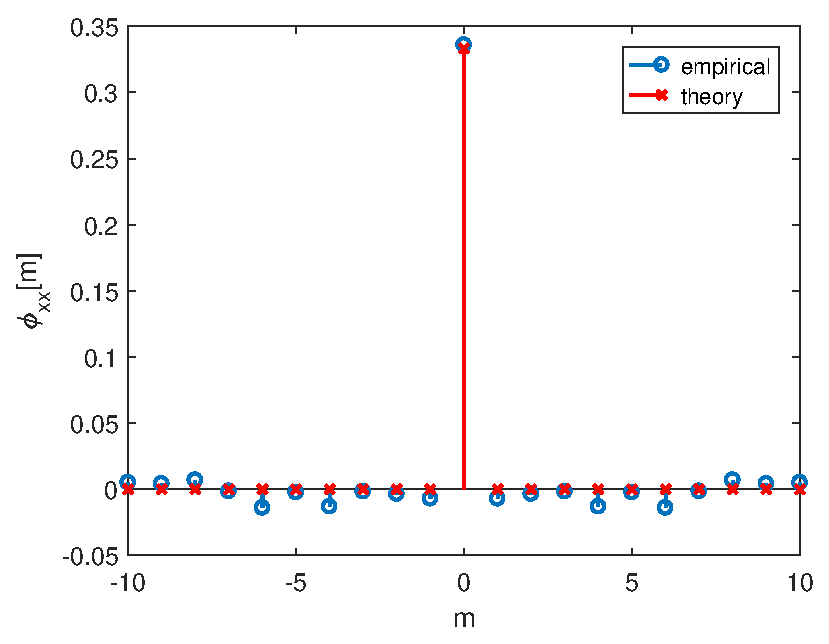
\includegraphics[width=\linewidth]{figs/lec2_random_experiment1_phi_xx.eps}
		\end{figure}
	}
	\only<3|handout:2>{
		\begin{figure}
			\centering
			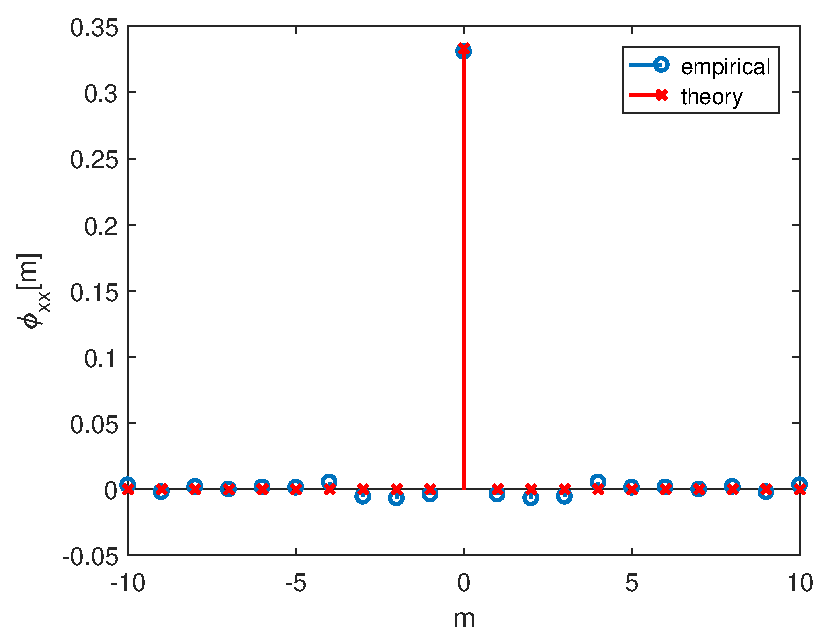
\includegraphics[width=\linewidth]{figs/lec2_random_experiment2_phi_xx.eps}
		\end{figure}
	}
	\end{column}

	\begin{column}{0.5\textwidth}
		\only<2|handout:1>{
		\begin{figure}
			\centering
			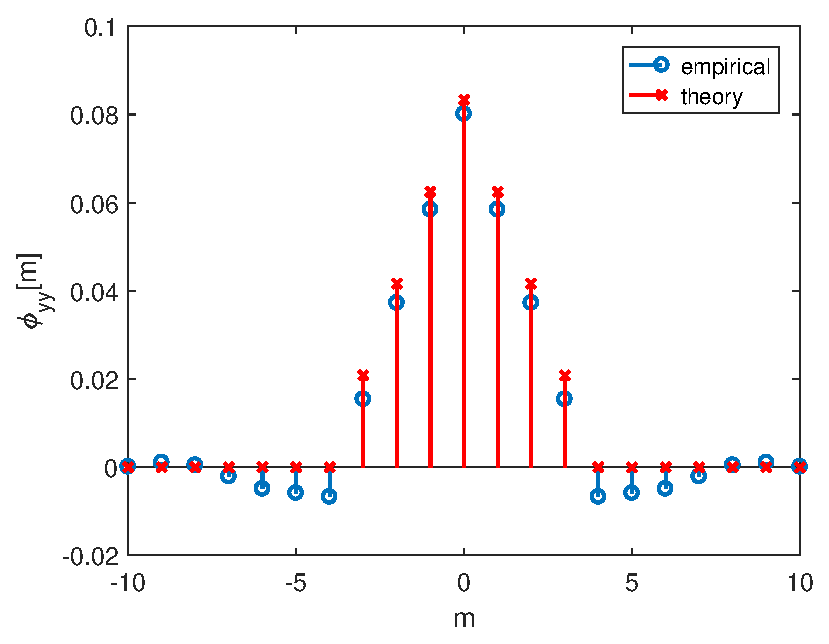
\includegraphics[width=\linewidth]{figs/lec2_random_experiment1_phi_yy.eps}
		\end{figure}
		}
		\only<3|handout:2>{
			\begin{figure}
				\centering
				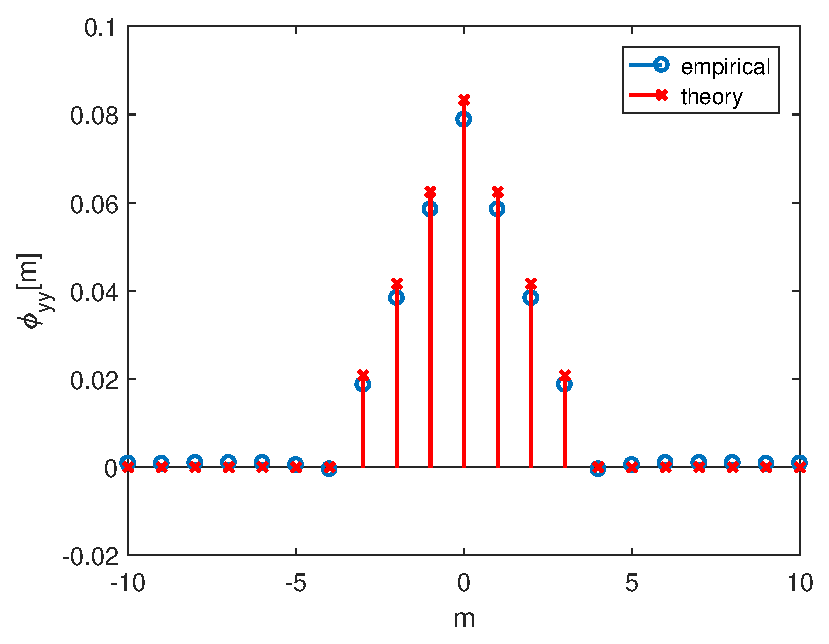
\includegraphics[width=\linewidth]{figs/lec2_random_experiment2_phi_yy.eps}
			\end{figure}
		}
	\end{column}
\end{columns}
\onslide<3|handout:2>{Now the random vector is $10000\times 1$}
\end{frame}

\begin{frame}{Estimating the probability density function}
\texttt{>> Nbins = 20} \\
\texttt{>> [counts, centers] = \textbf{hist}(x, Nbins)} \\
{\color{matlabcomment}\% normalize to make area under pdf equal to 1} \\
\texttt{>> x\_pdf = Nbins/(centers(end) - centers(1))*counts/sum(counts)} \\
\texttt{>> bar(centers, x\_pdf) {\color{matlabcomment}\% plot}}
\begin{columns}
	\begin{column}{0.5\textwidth}
			\begin{figure}
				\centering
				$p_x(x)$
				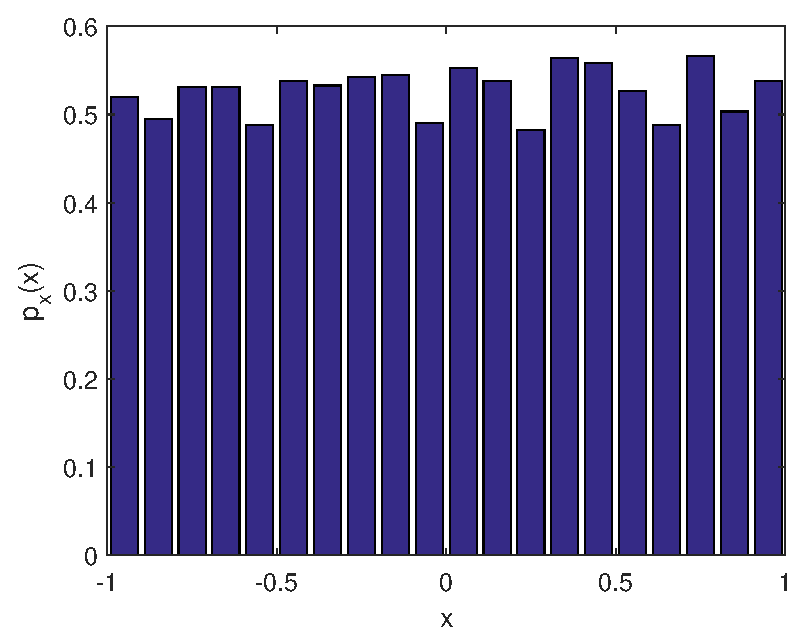
\includegraphics[width=\linewidth]{figs/lec2_random_experiment1_hist_x.eps}
			\end{figure}		
	\end{column}
	\begin{column}{0.5\textwidth}
	\begin{figure}
		\centering
		$p_y(y)$
		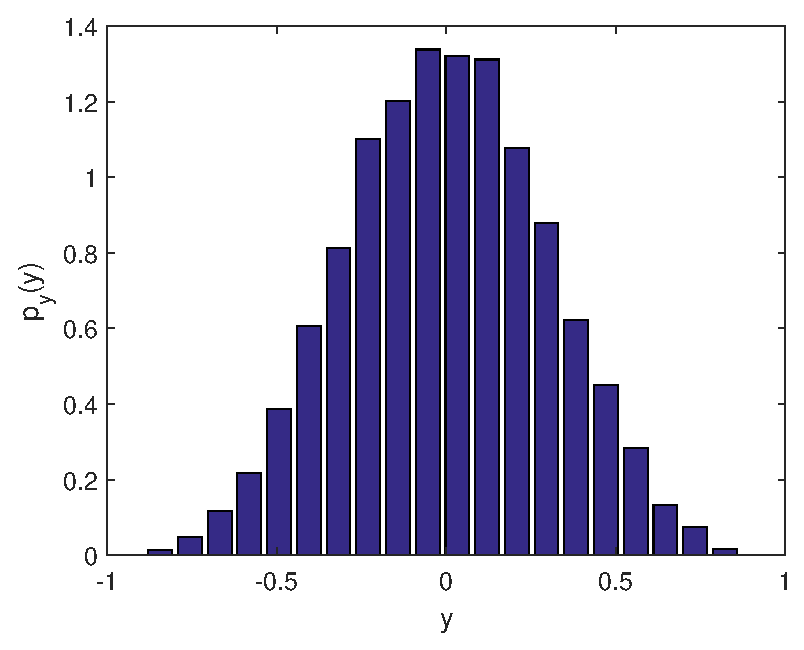
\includegraphics[width=\linewidth]{figs/lec2_random_experiment1_hist_y.eps}
	\end{figure}		
\end{column}
\end{columns}
\end{frame}

\begin{frame}{Central limit theorem}
The \textbf{central limit theorem} states that the probability density function of the sum of a large number of independent random variables approaches a Gaussian distribution.
\begin{equation*}
Z = X_1 + X_2 + \ldots + X_N \implies p_Z(z) \xrightarrow{N\to\infty} \mathcal{N}(\mu, \sigma^2)
\end{equation*}

\begin{itemize}
	\item In digital filters, we're essentially performing a weighted sum of samples of the input. As a result, the output of a digital filter for a random input is approximately Gaussian distributed.
	\item In the example of the 4-point moving average system, we were only adding 4 random variables and the resulting output pdf was close to Gaussian. 
	\item This effect is more visible in filters with larger memory, and in particular in filters with \textbf{infinite impulse response (IIR)} 
\end{itemize}

\end{frame}

\begin{frame}{Another probability theorem}

If we add two independent random variables $Z = X + Y$, the pdf of $Z$ is given by the convolution of the pdfs of $X$ and $Y$

\begin{equation*}
p_Z = p_X \ast p_Y
\end{equation*}

\pause
We can extend that to a sum of several independent random variables:
\begin{equation*}
Z = \sum_{k=1}^N X_k \implies p_Z = p_{X_1} \ast \ldots \ast p_{X_N}
\end{equation*}

\pause
From the \textbf{central limit theorem}, we know that as $N\to\infty$,  $p_Z\to\mathcal{N}(\mu, \sigma^2)$

\begin{itemize}
	\item This shows that the convolution of many signals $h_1(t) \ast h_2(t) \ast \ldots \ast h_N(t) \approx g(t)$, where $g(t)$ is the Gaussian function.
	\item Hence, if we cascade many LTI systems, the impulse response of the equivalent LTI system is approximately the Gaussian function.
\end{itemize}


\end{frame}

\begin{frame}{Summary}
\begin{itemize}
	%\item We use random processes to model signals that cannot be easily described by simple equations
	\item A random process is an indexed collection of random variables
	\item A random process is strict-sense stationary (SSS) if all its finite-order statistics are time invariant. That's hard to verify in practice.
	\item A random process is wide-sense stationary (WSS) if its mean is constant and if its autocorrelation function is only a function of the time difference. 
	\item A random process is ergodic if its time averages are equal to its probability averages
	\item The Fourier transform of the autocorrelation function is called the power spectrum density (PSD). The PSD has units of W/Hz or dBm/Hz.
	\item When a random signal is filtered by an LTI system defined by $h[n]\leftrightarrow H(e^j\omega)$, its autocorrelation function is filtered by an LTI system defined by $h[n]\ast h^*[-n]$, and its PSD is shaped by $|H(e^{j\omega})|^2$
	\item Random processes that have PSD constant over all frequencies are called white noise
	\item By the central limit theorem, the output of an LTI system to a random input is approximately Gaussian distributed
	
\end{itemize}
\end{frame}

\end{document}
